\documentclass[12pt]{article}

\usepackage{aircrafts_vi}
\title{\Large Phân tích năng lượng của mô hình ODE có điều khiển\\ với khối lượng biến thiên}
\newcommand{\authorinfo}{Khoa Toán - Tin học; e-mail: \texttt{2511001864@student.hcmus.edu.vn}\\
Tất cả mã nguồn Latex, mô phỏng số và tiến trình của báo cáo này
được lưu lại ở \url{https://github.com/aleksis-arendt/aircrafts}.}
\author{
  \normalsize Phạm Ngọc Gia Bảo\\
  \normalsize Đại học Khoa học Tự nhiên, ĐHQG-TPHCM\footnote{\authorinfo}
}
\date{\normalsize\today}

\makeatletter
\renewcommand{\@maketitle}{%
  \newpage
  \vspace*{-2cm}%
  \begin{center}%
  \let \footnote \thanks
    {\LARGE \@title \par}%
    \vskip 1.5em%
    {\large
      \lineskip .5em%
      \begin{tabular}[t]{c}%
        \@author
      \end{tabular}\par}%
    \vskip 1em%
    {\large \@date}%
  \end{center}%
  \par
  \vskip 1.5em}
\makeatother

\begin{document}

\maketitle
\begin{abstract}
Trong bài báo cáo này, ta khảo sát các mô hình ODE có điều khiển đơn giản hóa cho chuyển động một chiều dưới tác dụng của trọng lực, lực cản, điều khiển phản hồi và khối lượng biến thiên.
Sau đó, ta phân tích các phương trình sai số thu được bằng nghiệm đặc trưng và phương pháp năng lượng.
Ý tưởng này sau đó được mở rộng cho mô hình máy bay với hệ số giảm chấn phụ thuộc khối lượng và mô hình lực đẩy của tàu vũ trụ.
\end{abstract}
\tableofcontents

\section*{Giới thiệu}
Trong cơ học cổ điển, định luật II Newton cho ta mối liên hệ cơ bản giữa lực, khối lượng, vận tốc và gia tốc~\cite{arnold_classical_mechanics}, được viết dưới dạng
\[
 F = ma = m\dot v = m\ddot h.
\]
Để đơn giản hóa bài toán, ta đặt ra một số giả thiết. Mọi chuyển động được khảo sát đều là chuyển động một chiều. Trong Phần I, vật chuyển động có khối lượng không đổi. Hệ luôn chịu tác dụng của trọng lực, và lực cản phụ thuộc tuyến tính vào vận tốc. Ngoài ra, các chi tiết về khí động học, chuyển động quay, ràng buộc về hướng lực đẩy và nhiễu loạn đều được bỏ qua. 

Ta chọn một hệ tọa độ một chiều có chiều dương hướng lên. Giả sử độ cao của vật tại thời điểm $t$ là $h(t)$, và ta muốn vật tiến tới độ cao mong muốn $h_d$, là một hằng số. Theo định luật II Newton, chuyển động có thể được viết dưới dạng
\[
 h'(t) = v(t),\quad v'(t) = u(t) - g - cv(t).
\]
Phương trình thứ nhất nói rằng vận tốc là đạo hàm của độ cao, còn phương trình thứ hai cho biết gia tốc tăng do tín hiệu điều khiển và giảm do trọng lực cùng lực cản tuyến tính. Ta định nghĩa sai số bởi
\[
 e(t) = h(t) - h_d.
\]
Khi đó, bài toán ổn định trở thành câu hỏi $e(t)$ có tiến về 0 khi thời gian tăng hay không. Ta chọn tín hiệu điều khiển
\[
 u(t) = g - k_1e(t) - k_2v(t),
\]
trong đó $k_1$ và $k_2$ là các hằng số cần chọn, khi đó tín hiệu điều khiển được điều chỉnh theo sai số và vận tốc hiện tại. Thay vào phương trình trên cho ta được phương trình CLE (closed-loop error equation)
\[
 e'' + (k_2 + c)e' + k_1e = 0.
\]
Đây là một ODE tuyến tính cấp hai. Câu hỏi trung tâm là thông qua các tham số phản hồi, tín hiệu điều khiển ảnh hưởng thế nào đến tính ổn định và hành vi giảm chấn của vật được khảo sát.

Tất cả mã nguồn Latex, mô phỏng số và tiến trình của báo cáo này
được lưu lại ở \url{https://github.com/aleksis-arendt/aircrafts}.
\part{Mô hình ODE điều khiển và phân tích năng lượng}
\section{Mô hình chuyển động một chiều}

\subsection{Xây dựng mô hình}
Ký hiệu dùng trong mô hình một chiều được tóm tắt trong Bảng~\ref{tab:1d-notation}.

Ta chọn tọa độ thẳng đứng sao cho chiều dương hướng lên. Trong mô hình này, khối lượng của vật chuyển động $m$ được giả sử là hằng số, $g$ được xem là gia tốc trọng trường không đổi, và độ cao mong muốn $h_d$ là cố định. Lực cản phụ thuộc tuyến tính vào vận tốc của vật, cụ thể là

\[
 F_{\mathrm{drag}} = -bv.
\]
Để đơn giản, ta bỏ qua lực cản phi tuyến, lực nâng, chuyển động quay, ràng buộc hướng lực đẩy, nhiễu loạn và sự biến thiên khối lượng.

Các lực tác dụng lên vật bao gồm lực đẩy $T(t)$, trọng lực $-mg$, và lực cản tuyến tính $-bv(t)$. Theo định luật II Newton~\cite{arnold_classical_mechanics}, ta có
\[
 m h''(t) = T(t) - mg - bv(t).
\]
Vì $v(t) = h'(t)$, ta có thể viết lại thành
\begin{equation}\label{eq:newton-motion}
 T(t) - mg - bh'(t) = m h''(t).
\end{equation}

\begin{figure}[h]
\centering
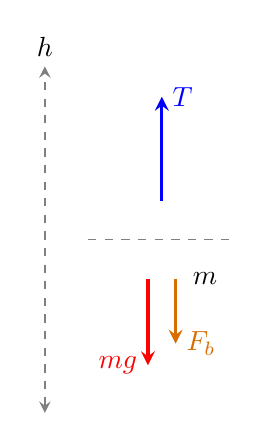
\begin{tikzpicture}[scale=1.1,>=stealth]
    \draw[<->,thick,dashed,gray] (-1.35,-2.0) -- (-1.35,2)
        node[above,black] {$h$};
    \draw[dashed,gray] (-0.85,0) -- (0.85,0);
    \node[scale=2.6,rotate=90] at (0,0) {\Plane};
    \node at (0.5,-0.45) {$m$};

    \draw[->,very thick,blue] (0,0.45) -- (0,1.65)
        node[right,blue] {$T$};
    \draw[->,very thick,red] (-0.16,-0.45) -- (-0.16,-1.45)
        node[left,red] {$mg$};
    \draw[->,very thick,orange!85!black] (0.16,-0.45) -- (0.16,-1.2)
        node[right,orange!85!black] {$F_b$};

\end{tikzpicture}
\caption{Các lực trong mô hình thẳng đứng.}
\end{figure}
Ta định nghĩa tín hiệu điều khiển chuẩn hóa và hệ số cản lần lượt là
$u(t) = \frac{T(t)}{m},$ và $c = \frac{b}{m}.$
Chia \eqref{eq:newton-motion} cho $m$ ta được
\begin{equation}\label{eq:normalized-motion}
 h''(t) = u(t) - g - cv(t).
\end{equation}
Đặt $v(t) = h'(t)$, phương trình trên trở thành
\begin{equation}\label{eq:motion-system}
\boxed{
\begin{cases}
 h'(t) = v(t),\\
 v'(t) = u(t) - g - cv(t).
\end{cases}
}
\end{equation}

Hằng số $c = b/m$ là hệ số cản tuyến tính chuẩn hóa.
Vì hạng tử $-cv(t)$ trái dấu với vận tốc, nó luôn chống lại hướng chuyển động.

\subsection{Sai số và tín hiệu điều khiển}
Cho $h_d$ là độ cao mong muốn. Mục tiêu là thiết kế một tín hiệu điều khiển  $u(t)$ sao cho độ cao $h(t) \to h_d$ theo thời gian. Để đo độ lệch giữa độ cao hiện tại và độ cao mong muốn, ta định nghĩa \textit{sai số } $e(t) = h(t) - h_d.$ Khi đó, bài toán ổn định trở thành bài toán chọn $u(t)$ sao cho $e(t) \to 0$ khi $t \to + \infty$. Việc chọn $u(t)$ được cân nhắc bởi các yêu cầu sau:

Thứ nhất, tín hiệu điều khiển nên phụ thuộc vào trạng thái hiện tại của hệ, đặc biệt là sai số $e(t)$ và vận tốc $v(t)$.

Thứ hai, nếu vật ở trên độ cao mong muốn, tức là $e(t) > 0$, tín hiệu điều khiển nên giảm để kéo vật đi xuống. Nếu vật ở dưới độ cao mong muốn, tức là $e(t) < 0$, tín hiệu điều khiển nên tăng để đẩy vật đi lên. Điều này dẫn đến hạng tử hiệu chỉnh tỉ lệ có dạng $-k_1e(t)$.

Thứ ba, chỉ điều khiển sai số vị trí là chưa đủ để tránh vượt quá mục tiêu. Khi vật ở gần độ cao mong muốn nhưng vẫn chuyển động nhanh, tín hiệu điều khiển cũng cần phản ứng với vận tốc. Nếu $v(t) > 0$, vật đang đi lên và tín hiệu điều khiển nên giảm; nếu $v(t) < 0$, vật đang đi xuống và tín hiệu điều khiển nên tăng. Điều này dẫn đến hạng tử hiệu chỉnh đạo hàm có dạng $-k_2v(t)$, bổ sung giảm chấn cho hệ.

Cuối cùng, khi vật ở độ cao mong muốn và đứng yên, tức là khi $e(t) = 0$ và $v(t) = 0$, ta muốn nó giữ nguyên vị trí thay vì rơi do trọng lực~\cite[Ch.~1]{yanushevsky2019modern}. Phương trình
\[
 v' = u - g - cv,
\] 
đòi hỏi $u = g$ tại cân bằng. Vì vậy, ta đưa vào hạng tử bù trọng lực $g$ và chọn 
\[
 u(t) = g - k_1e(t) - k_2v(t),
\]
trong đó $k_1, k_2 > 0$ là các hệ số phản hồi. Tham số $k_1$ quyết định bộ điều khiển phản ứng mạnh thế nào với sai số vị trí, còn $k_2$ quyết định mức giảm chấn đối với vận tốc. Vì $v(t) = e'(t)$, ta có thể viết lại~\eqref{eq:motion-system} theo $e(t)$ dưới dạng
\begin{equation}\label{eq:main}
 \boxed{e''(t) + (k_2 + c)e'(t) + k_1e(t) = 0.}
\end{equation}
Ta gọi phương trình này là \textit{phương trình sai số vòng kín}, gọi tắt là \textit{phương trình CLE} (closed-loop error equation).
\subsection{Mô phỏng số}
Để minh họa tác động của tín hiệu điều khiển $u$, ta mô phỏng mô hình trên bằng phương pháp RK4 và trực quan hóa kết quả bằng Matplotlib.
Chọn độ cao mong muốn là $h_d = 10,$ và các tham số 
\[
 g = 9.81, k_1 = 2, k_2 = 2.5, c = 0.3.
\] Ta so sánh ba trường hợp tiêu biểu.
\begin{center}
  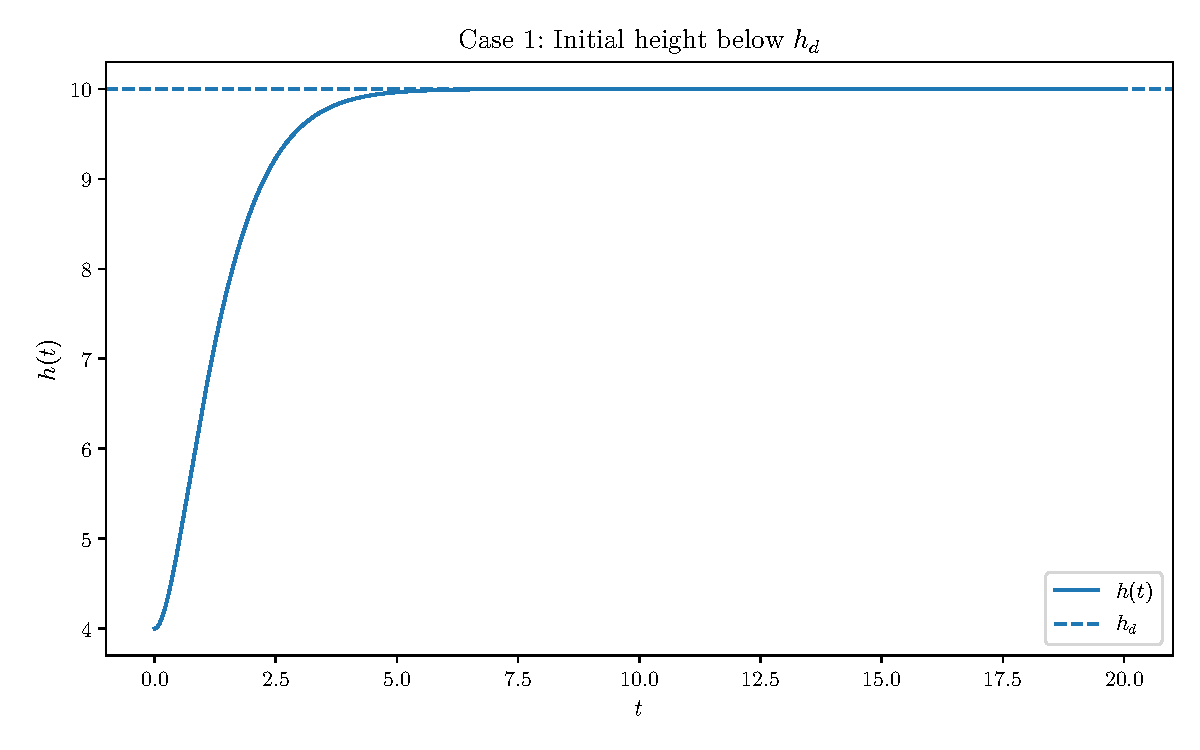
\includegraphics[scale=0.5]{figures/fig-02-02-case-01-below-hd.pdf}
\end{center}
Trong trường hợp thứ nhất, vật bắt đầu ở dưới độ cao mong muốn

\[
 h(0) = 4, v(0) = 0.
\]
Do sai số âm, luật phản hồi 

\[
 u = g - k_1(h - h_d) - k_2v
\]
làm tăng đầu vào điều khiển. Kết quả là độ cao tăng và tiến tới $h_d$.

\begin{center}
  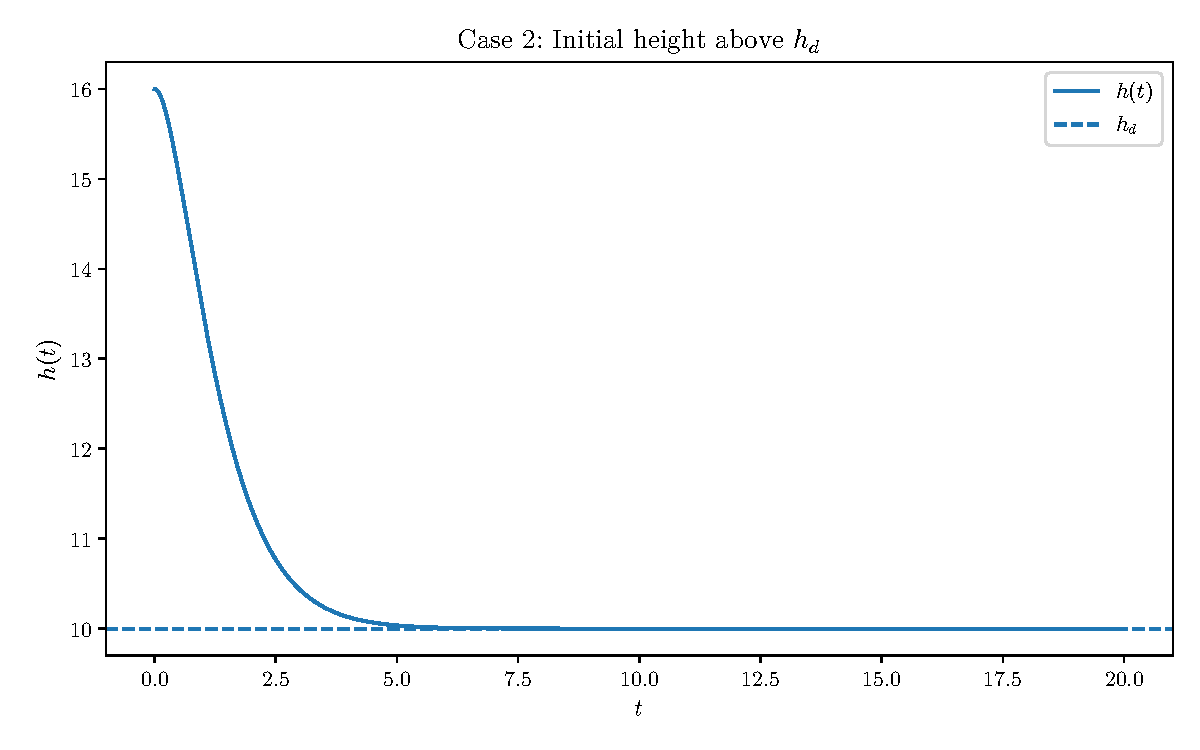
\includegraphics[scale=0.5]{figures/fig-02-02-case-02-above-hd.pdf}
\end{center}
Trong trường hợp thứ hai, vật bắt đầu ở trên độ cao mong muốn:
$h(0) = 16, v(0) = 0.$ Vì sai số dương, hạng tử phản hồi tỉ lệ làm giảm tín hiệu điều khiển. Sau đó độ cao giảm và tiến tới $h_d$.
\begin{center}
  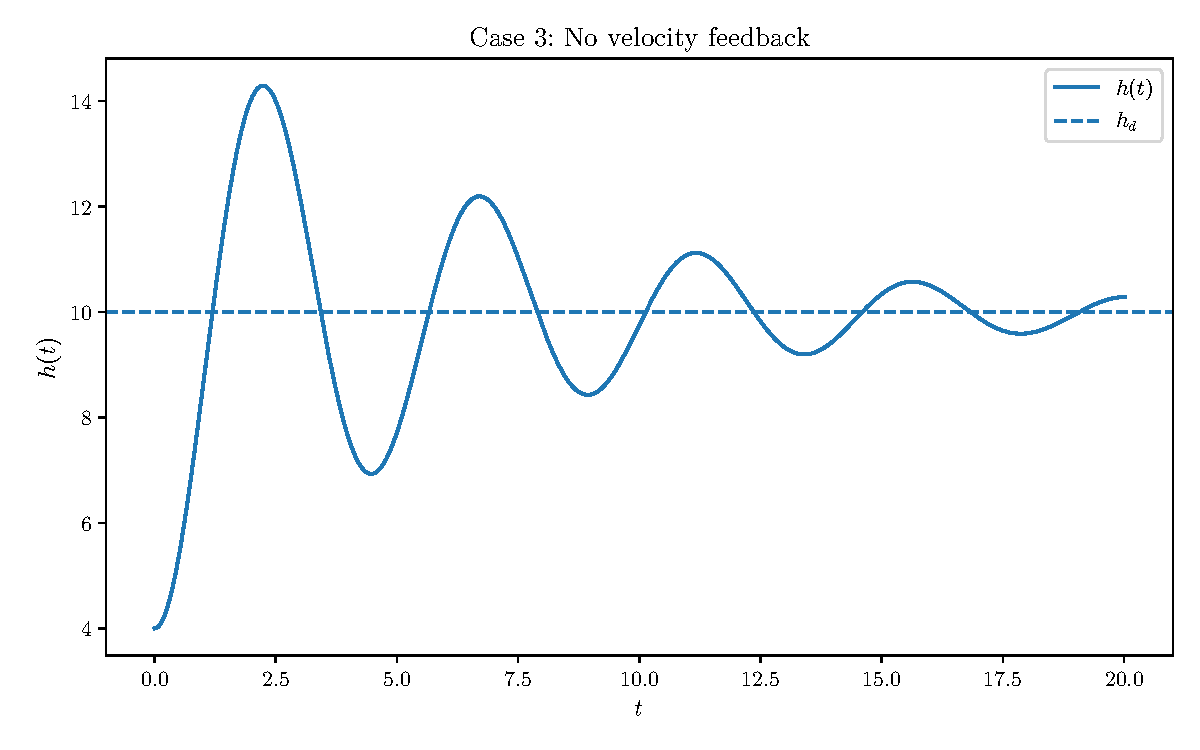
\includegraphics[scale=0.5]{figures/fig-02-02-case-03-no-velocity-feedback.pdf}
\end{center}
Trong trường hợp thứ ba, ta bỏ hạng tử phản hồi vận tốc và dùng
\[
 u = g - k_1(h - h_d).
\]
Điều này có nghĩa là bộ điều khiển chỉ phản ứng với sai số vị trí và không trực tiếp giảm chấn vận tốc. Mô phỏng cho thấy dao động mạnh hơn quanh $h_d$, minh họa vai trò của hạng tử đạo hàm $-k_2v$ như một cơ chế giảm chấn bổ sung.
\subsection{Phân tích ổn định của phương trình CLE}
\begin{theorem}
  
Đặt $\gamma = k_2 + c$, viết lại~\eqref{eq:main}, ta có
\begin{equation}\label{mainrewrite1}
 e''(t) + \gamma e'(t) + k_1 e(t) = 0.
\end{equation}
Giả sử $k_1 > 0$ và $\gamma > 0$. Nếu $e(t)$ là nghiệm của~\eqref{mainrewrite1}, thì $\limit_{t \to + \infty} e(t) = 0$.
\end{theorem}
\begin{proof} Xét phương trình đặc của~\eqref{mainrewrite1}:
\begin{equation}\label{characteristic}
 \lambda^2 + \gamma\lambda + k_1 = 0,
\end{equation}
Biệt thức của~\eqref{characteristic} là
$\Delta = \gamma^2 - 4k_1.$
Ta biện luận dấu của $\Delta$.

\textbf{Trường hợp 1: $\Delta > 0$.} Phương trình đặc trưng có hai nghiệm thực phân biệt

\[
 \lambda_1,\lambda_2 = \frac{-\gamma \pm \sqrt{\Delta}}{2}.
\]
Theo công thức Viète, ta có
\[
 \begin{cases}
 \lambda_1 + \lambda_2 = -\gamma < 0,\\
 \lambda_1\lambda_2 = k_1 > 0.
 \end{cases}
\]
Vì vậy cả hai nghiệm đều âm. Nghiệm tổng quát là
\[
 e(t) = Ae^{\lambda_1 t} + Be^{\lambda_2 t},
\]
trong đó $A, B \in \mathbb R$ được xác định bởi dữ kiện ban đầu. Vì
$\lambda_1 < 0,\lambda_2 < 0,$ nên ta được giới hạn
$\limit_{t \to + \infty} e(t) = 0.$
Đây là trường hợp tắt dần hoàn toàn, trong đó sai số hội tụ về không mà không dao động.

\textbf{Trường hợp 2: $\Delta = 0$.} Phương trình đặc trưng có nghiệm thực kép
$\lambda = -\frac{\gamma}{2}.$ Nghiệm tổng quát là
\[
 e(t) = (A + Bt)e^{-\gamma t/2}.
\]
Vì $\gamma > 0$, nhân tử mũ $e^{-\gamma t/2}$ trội hơn nhân tử tuyến tính $A + Bt$. Do đó,
\[
 \lim_{t \to + \infty} e(t) = 0.
\]
Đây là trường hợp tắt dần tới hạn, có thể hội tụ không dao động hoặc hội tụ có dao động.

\textbf{Trường hợp 3: $\Delta < 0$.} Các nghiệm đặc trưng là một cặp số phức liên hợp:
\[
 \lambda_{\pm} = -\frac{\gamma}{2} \pm i\omega,\quad \omega = \frac{\sqrt{4k_1 - \gamma^2}}{2}.
\]
Nghiệm thực tổng quát là
\[
 e(t) = e^{-\gamma t/2} \left( A\cos(\omega t) + B\sin(\omega t) \right).
\]
Dùng ước lượng
\[
 \left|A\cos(\omega t) + B\sin(\omega t)\right| \leq \sqrt{A^2 + B^2},
\]
ta được
\[
 |e(t)| \leq \sqrt{A^2 + B^2}\, e^{-\gamma t/2} \to 0
\]
khi $t \to + \infty$. Do đó, $\limit_{t \to + \infty} e(t) = 0$.
\end{proof}

Ví dụ, với $k_1 = 4$, $e(0) = 3$, và $e'(0) = 0$, ba giá trị
$\gamma = 5, 4, 1.2$ lần lượt cho các hành vi tắt dần hoàn toàn, tắt dần tới hạn và dao động tắt dần như hình dưới. 
\begin{center}
  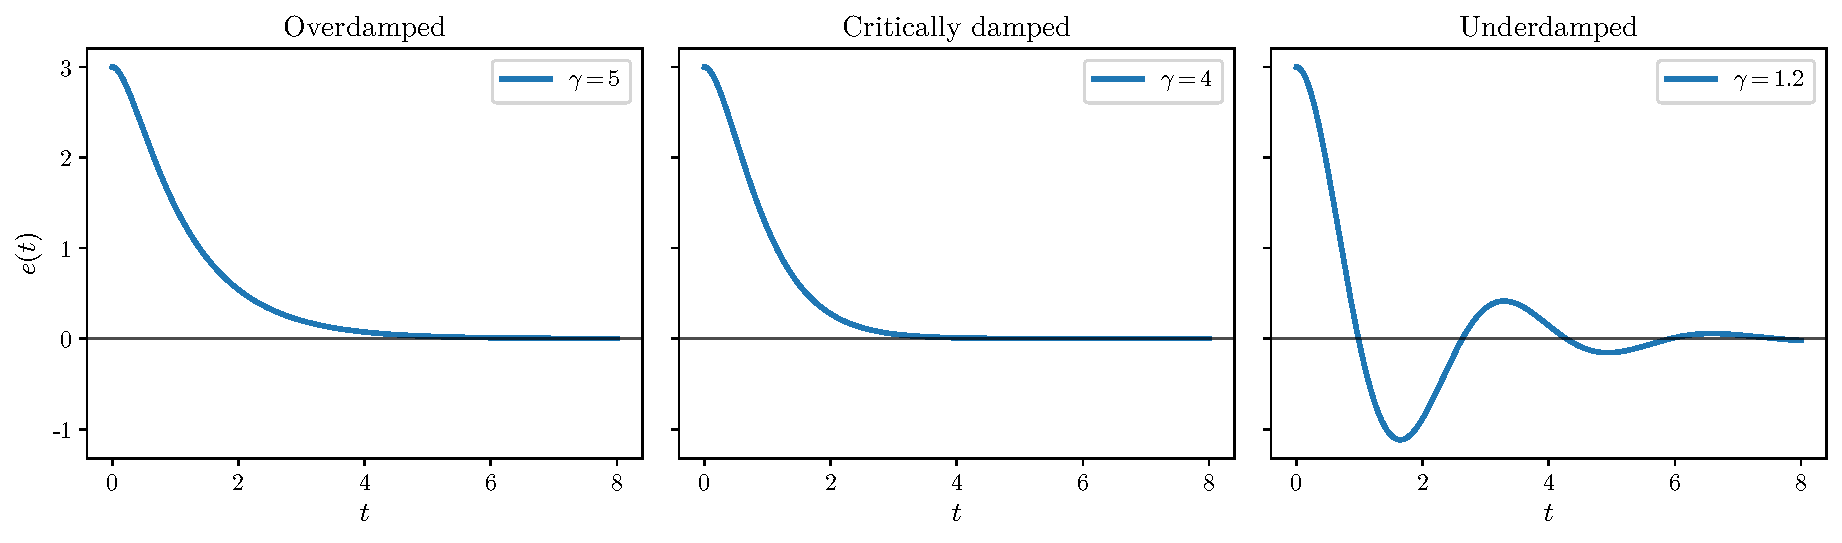
\includegraphics[scale=0.5]{figures/fig-02-05-three-regimes-side-by-side.pdf}
\end{center}

Trong cả ba trường hợp, giả thiết $k_1 > 0,\gamma = k_2 + c > 0$
bảo đảm rằng sai số luôn thỏa mãn $e(t) \to 0$.
Do đó, độ cao $h(t)$ tiến tới độ cao mong muốn $h_d$.

Tuy nhiên, nghiệm đặc trưng chỉ mô tả hành vi tiệm cận của nghiệm mà không trực tiếp đo lượng năng lượng sai số còn lại trong hệ hoặc tốc độ tiêu tán của năng lượng này. Để nghiên cứu hành vi đó rõ hơn, ta chuyển sang khảo sát các khía cạnh năng lượng của hệ.
\section{Phương pháp năng lượng cho phương trình CLE}
Ký hiệu dùng cho phần năng lượng và công thức biến phân được tóm tắt trong Bảng~\ref{tab:energy-notation}.
\subsection{Năng lượng trạng thái sai số}
Trong phần này, ta xét một hàm năng lượng đo độ lớn của sai số theo thời gian~\cite[Sec.~5.3, pp.~59--61]{yanushevsky2019modern}. Một đại lượng như vậy cần thỏa mãn vài yêu cầu.

Thứ nhất, đại lượng này nên đo cả hai thành phần sai số $e(t)$ và vận tốc sai số $e'(t)$ trong phương trình CLE. 

Thứ hai, nó phải không âm và chỉ bằng không tại trạng thái cân bằng $e = e' = 0.$

Thứ ba, đạo hàm của đại lượng đó nên chứa nhân tử $(e'' + k_1e)$  để phương trình CLE biến nó thành một hạng tử tiêu tán.

Những cân nhắc trên dẫn đến lựa chọn
\[
 \boxed{E(t) = \frac{1}{2}(e'(t))^2 + \frac{1}{2}k_1e(t)^2.}
\]
Ta gọi đây là \textit{năng lượng trạng thái sai số}. Hạng tử thứ nhất đo phần vận tốc của sai số, còn hạng tử thứ hai đo phần vị trí của sai số. Do đó, về mặt biểu thức, năng lượng này cho biết trạng thái sai số lớn đến mức nào tại thời điểm $t$.
\begin{lemma}\label{decreasing}
  Với mọi $t > 0$, ta có $E'(t) = -\gamma (e'(t))^2$.
\end{lemma}
\begin{proof}
  Tính trực tiếp và dùng~\eqref{mainrewrite1}, ta được
  \begin{align*}
 E'(t) = e''(t)e'(t) + k_1 e'(t)e(t) = e'(t)(e''(t) + k_1e(t)) = e'(t) [-\gamma e'(t)]
 \end{align*}
  Do đó $E'(t) = -\gamma (e'(t))^2$ với mọi $t > 0$.
\end{proof}

Từ bổ đề này, ta thấy năng lượng sai số không tăng theo thời gian. Vì vậy hệ CLE không tạo thêm năng lượng sai số; ngược lại, hạng tử giảm chấn $\gamma e'$ tiêu tán nó.

Để so sánh các lựa chọn phản hồi khác nhau trên một khoảng thời gian, ta đưa vào \textit{năng lượng sai số tích lũy}
\[
 J_E(T) = \int_0^T E(t)\, dt.
\]
Đối với năng lượng sai số tích lũy trên toàn bộ khoảng thời gian, ta định nghĩa
\[
 J_E:= \lim_{T \to + \infty} \int_0^T E(t)dt = \int_0^\infty E(t)dt.
\]
\subsection{Chi phí điều khiển tích lũy}
Chỉ tối ưu $J_E$  có thể dẫn tới tín hiệu điều khiển rất lớn.
Để đo độ lớn của tín hiệu, ta thấy tín hiệu điều khiển có thể được tách thành hai phần:
\[
 u(t) = \underbrace{g}_{\text{bù trọng lực}} + \underbrace{\bigl(-k_1e(t) - k_2e'(t)\bigr)}_{\text{hiệu chỉnh phản hồi}}.
\]
Hạng tử $g$ được thêm vào để bù trọng lực. Thật vậy, khi vật ở đúng độ cao mong muốn và đứng yên, ta có $e(t) = e'(t) = 0$,
nhưng vẫn phải có $u(t) = g$ để giữ vật không rơi. Do đó, $g$ không phải phần hiệu chỉnh dùng để giảm sai số. Vì lý do này, ta đo phần hiệu chỉnh phản hồi ngoài bù trọng lực
\[
 u(t) - g = -k_1e(t) - k_2e'(t) = e''(t) + ce'(t)
\]
Khi đó \textit{chi phí điều khiển tích lũy} được định nghĩa bởi
\[
 J_u = \int_0^T (u(t) - g)^2\, dt.
\]
Đại lượng này đo tổng độ lớn của tín hiệu hiệu chỉnh trên khoảng thời gian $[0, T]$. Nếu hệ đã ở cân bằng, thì $u(t) - g = 0$, và do đó $J_u = 0$.
\subsection{Công thức biến phân cho chi phí hiệu năng}\label{VF}

Năng lượng sai số tích lũy $J_E$ đo mức độ trạng thái sai số còn tồn tại theo thời gian, còn chi phí điều khiển tích lũy $J_u$ đo lượng tín hiệu hiệu chỉnh mà bộ điều khiển sử dụng. Để cân bằng hai hiệu ứng này, ta đưa vào phiếm hàm chi phí hiệu năng kết hợp
\[
 \boxed{ J[e] = \int_0^T \left[ \frac{1}{2}q e(t)^2 + \frac{1}{2}p(e'(t))^2 + \frac{1}{2}r(e''(t) + ce'(t))^2 \right]dt,}
\]
trong đó $q, p, r > 0$. Hạng tử thứ nhất phạt sai số vị trí, hạng tử thứ hai phạt sai số vận tốc, và hạng tử thứ ba phạt chi phí điều khiển hiệu chỉnh.
Lagrangian của phiếm hàm trên là
\[
 L(e, e', e'') = \frac{1}{2}q e^2 + \frac{1}{2}p(e')^2 + \frac{1}{2}r(e'' + ce')^2.
\]
Vì $L$ phụ thuộc vào $e''$, ta dùng phương trình Euler--Lagrange bậc cao từ phép tính biến phân~\cite{rindler2018calculus}. Kết quả này được phát biểu và chứng minh trong Phụ lục~\ref{append1}. Phương trình Euler--Lagrange trong bài toán này là
\[
 \frac{\partial L}{\partial e} - \frac{d}{dt}\left(\frac{\partial L}{\partial e'}\right) + \frac{d^2}{dt^2}\left(\frac{\partial L}{\partial e''}\right) = 0.
\]
Ta tính từng hạng tử riêng. Trước hết, ta có 
\[
 \frac{\partial L}{\partial e} = qe.
\]
Tiếp theo, vì
\[
 L = \frac{1}{2} q e^2 + \frac{1}{2} p(e')^2 + \frac{1}{2} r(e'' + ce')^2,
\]
ta có
\[
 \frac{\partial L}{\partial e'} = pe' + rc(e'' + ce').
\]
Do đó,
\[
\begin{aligned}
 \frac{d}{dt}\left(\frac{\partial L}{\partial e'}\right)
 & = \frac{d}{dt} \left[ pe' + rc(e'' + ce') \right]\\
 & = pe'' + rc(e''' + ce'').
\end{aligned}
\]
Tương tự,
\[
 \frac{\partial L}{\partial e''} = r(e'' + ce'),
\]
và vì vậy
\[
\begin{aligned}
 \frac{d^2}{dt^2}\left(\frac{\partial L}{\partial e''}\right)
 & = \frac{d^2}{dt^2} \left[ r(e'' + ce')\right]\\
 & = r(e^{(4)} + ce''').
\end{aligned}
\]
Thay các biểu thức này vào phương trình Euler--Lagrange cho ta
\[
 qe - \left[ pe'' + rc(e''' + ce'') \right] + r(e^{(4)} + ce''') = 0.
\]
Khai triển các hạng tử, ta được
\[
 qe - pe'' - rce''' - rc^2e'' + re^{(4)} + rce''' = 0.
\]
 Vì vậy,
\[
 \boxed{ re^{(4)} - (p + rc^2)e'' + qe = 0. }
\]
Đối với một bài toán biên đơn giản, ta có thể giả sử
\[
 e(0) = e_0,\quad e'(0) = w_0,\quad e(T) = 0,\quad e'(T) = 0
\]

Cuối cùng, bổ đề~\ref{minimizer} cho thấy nghiệm của phương trình này là cực tiểu toàn cục duy nhất của phiếm hàm hiệu năng.
\subsection{Định lý phân tích nhân tử}
Phương trình Euler--Lagrange gắn với phiếm hàm biến phân là
\[
 re^{(4)} - (p + rc^2)e'' + qe = 0.
\]
Viết $D = d/dt$, phương trình này có dạng toán tử
\begin{equation}\label{eq:el-operator}
 \left[rD^4 - (p + rc^2)D^2 + q\right]e = 0.
\end{equation}
Mặt khác, phương trình CLE sinh bởi một tín hiệu điều khiển là
\[
 e'' + \gamma e' + k_1e = 0,
\]
trong đó $\gamma = k_2 + c$. Tương đương,
\begin{equation}\label{eq:cle-operator}
 (D^2 + \gamma D + k_1)e = 0.
\end{equation}
Các tính chất cần thiết cho các biến đổi toán tử đại số được phát biểu và chứng minh trong Phụ lục~\ref{appendix:operator-algebra}.

\begin{theorem}[Định lý phân tích nhân tử]\label{factor}
Giả sử $p, q, r > 0$, $k_1 > 0$, và $\gamma = k_2 + c > 0$.
Mọi nghiệm của~\eqref{eq:cle-operator} cũng thỏa~\eqref{eq:el-operator} khi và chỉ khi
\[
 k_1 = \sqrt{\frac{q}{r}} \quad \text{và}\quad k_2 = \sqrt{ \frac{p}{r} + c^2 + 2\sqrt{\frac{q}{r}} } - c.
\]
\end{theorem}

\begin{proof}
Đặt
\[
 P(\lambda) = \lambda^2 + \gamma\lambda + k_1\quad\text{và}\quad
 Q(\lambda) = r\lambda^4 - (p + rc^2)\lambda^2 + q.
\]
Ta có
$
 \ker P(D) \subseteq \ker Q(D)
$. Theo Bổ đề~\ref{lem:operator-kernel-inclusion}, điều này tương đương với $P \mid Q$.
Do đó tồn tại một đa thức $R$ sao cho
\[
 Q(\lambda) = R(\lambda)P(\lambda).
\]
Vì $\deg Q = 4$ và $\deg P = 2$, thương có bậc $2$. Viết
\[
 R(\lambda) = r\lambda^2 + A\lambda + B.
\]Khai triển tích $R(\lambda)P(\lambda)$, ta được
\[
\begin{aligned}
 R(\lambda)P(\lambda)
 & = (r\lambda^2 + A\lambda + B)(\lambda^2 + \gamma\lambda + k_1)\\
 & = r\lambda^4 + (r\gamma + A)\lambda^3 + (rk_1 + A\gamma + B)\lambda^2\\
 &\quad + (Ak_1 + B\gamma)\lambda + Bk_1.
\end{aligned}
\]
So sánh với đa thức
\[
 Q(\lambda) = r\lambda^4 - (p + rc^2)\lambda^2 + q = R(\lambda)P(\lambda),
\]
ta thu được
\[
 A = -r\gamma \quad \text{ và }B = rk_1.
\]
Khi đó
\[
 r(D^2 - \gamma D + k_1)(D^2 + \gamma D + k_1) = rD^4 + r(2k_1 - \gamma^2)D^2 + rk_1^2.
\]
Ta so sánh toán tử này với~\eqref{eq:el-operator}:
\[
\begin{cases}
 rk_1^2 = q,\\
 r(2k_1 - \gamma^2) = -(p + rc^2).
\end{cases}
\]
Vì $r > 0$, $q > 0$, và $k_1 > 0$, phương trình thứ nhất cho
\[
 k_1 = \sqrt{\frac{q}{r}}.
\]
Từ phương trình thứ hai, ta có
\[
 \gamma^2 = \frac{p}{r} + c^2 + 2k_1.
\]
Thay $k_1 = \sqrt{q/r}$, ta được
\[
 (k_2 + c)^2 = \gamma^2 = \frac{p}{r} + c^2 + 2\sqrt{\frac{q}{r}}.
\]
Vì $\gamma > 0$, suy ra
\[
 k_2 = \sqrt{ \frac{p}{r} + c^2 + 2\sqrt{\frac{q}{r}} } - c.
\]
Ngược lại, nếu $k_1$ và $k_2$ được chọn theo các công thức này, thì
\[
 Q(\lambda) = r(\lambda^2 - \gamma\lambda + k_1)(\lambda^2 + \gamma\lambda + k_1).
\]
Vì vậy $P\mid Q$. Theo Bổ đề~\ref{lem:operator-kernel-inclusion}, ta thu được
$\ker P(D) \subseteq \ker Q(D)$.

Do đó mọi nghiệm của phương trình CLE cũng thỏa phương trình Euler--Lagrange. Chứng minh hoàn tất.
\end{proof}
Vì vậy, với lựa chọn $k_1$ và $k_2$ này, mọi quỹ đạo sinh bởi phương trình CLE tự động thỏa phương trình Euler--Lagrange. Trong các mô phỏng đơn giản, ta có thể cố định $r = 1$ như một thang tham chiếu rồi tinh chỉnh $p$ và $q$.
Một cách tiếp cận phổ biến khác là chuẩn hóa thang đo.
Nếu kích thước kỳ vọng của $e$, $e'$, và $e'' + ce'$ lần lượt là $E_0$, $v_{\mathrm{start}}$, và $A_0$, thì ta có thể chọn
\[
 q = \frac{1}{E_0^2},\quad p = \frac{1}{v_{\mathrm{start}}^2},\quad r = \frac{1}{A_0^2}.
\]
Cách chọn này làm cho ba hạng tử trong phiếm hàm hiệu năng có kích thước so sánh được và tránh việc một hạng tử chi phối chỉ vì đơn vị vật lý của nó.

\subsection{So sánh nghiệm biến phân và nghiệm thông thường của CLE}

Trong mục này, ta so sánh bằng mô phỏng số một số quỹ đạo của phương trình CLE.
Mọi quỹ đạo đều thu được bằng cách giải phương trình CLE
\[
 e'' + (k_2 + c)e' + k_1e = 0.
\]
Để áp dụng phương pháp số RK4, ta viết lại phương trình cấp hai này thành hệ cấp một
\[
 x_1 = e,\quad x_2 = e',
\]
sao cho
\[
\begin{cases}
 x_1' = x_2,\\
 x_2' = -(k_2 + c)x_2 - k_1x_1.
\end{cases}
\]
Ví dụ, ta chọn
\[
 q = 1,\quad p = 1,\quad r = 0.2,\quad c = 0.3.
\]
Định lý~\ref{factor} cho ta biết
\[
 k_1 = \sqrt{\frac{q}{r}},\quad k_2 = \sqrt{ \frac{p}{r} + c^2 + 2\sqrt{\frac{q}{r}} } - c.
\]
Do đó 
\[
 k_1 = \sqrt{5}\approx 2.2361,\quad \text{ và }\quad k_2 = \sqrt{ 5 + 0.09 + 2\sqrt5 } - 0.3 \approx 2.7923.
\]
Để so sánh, ta chọn thêm các bộ số
\[
 (k_1, k_2) = (4, 1), (4, 4), (4, 8).
\]
Mọi quỹ đạo đều bắt đầu từ cùng trạng thái sai số ban đầu
\[
 e(0) = 3,\quad e'(0) = 0,
\]
với độ cao mong muốn $h_d = 10$. Do đó
$h(0) = h_d + e(0) = 13$.
Đường cong sinh bởi
\[
 (k_1, k_2)\approx(2.2361, 2.7923)
\]
là quỹ đạo được sinh bởi các trọng số biến phân $p, q, r$.  Trường hợp $k_2 = 1$ có giảm chấn yếu và vượt xuống dưới độ cao mong muốn. Trường hợp $k_2 = 4$ tiến tới $h_d$ trơn tru hơn. Trường hợp $k_2 = 8$ có giảm chấn mạnh hơn và nằm phía trên $h_d$ trong thời gian dài hơn.
\begin{center}
    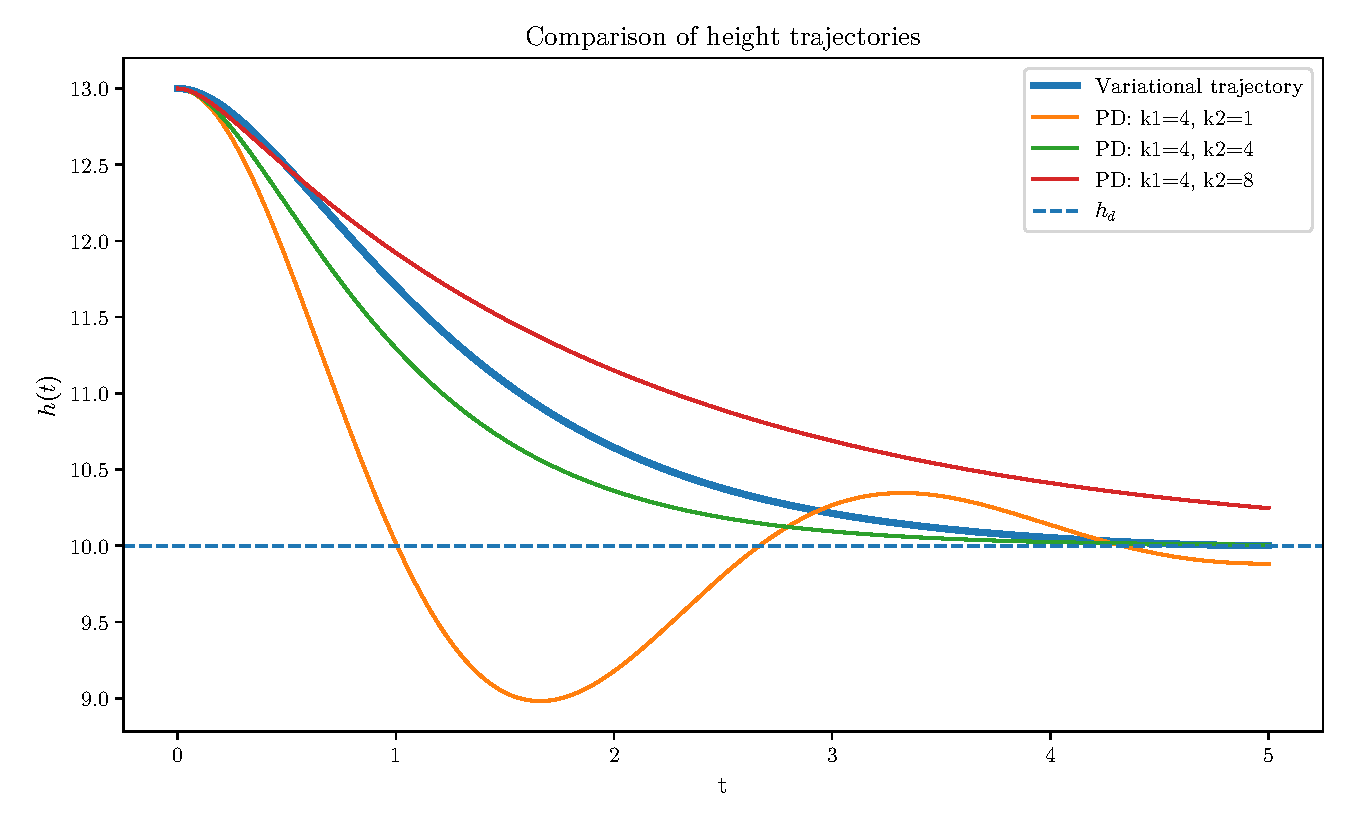
\includegraphics[scale=0.6]{figures/fig-02-07-variational-shooting.pdf}
\end{center}

\part{Ứng dụng với khối lượng biến thiên}
\section{Mô hình nhiên liệu và khối lượng của máy bay}

Những ký hiệu dùng trong mô hình này được tóm tắt trong Bảng~\ref{tab:fuel-notation}.

\begin{figure}[h]
\centering
\begin{tikzpicture}[scale=0.95,>=stealth]
    % đường băng và đường hạ độ cao
    \draw[thick] (-4.6,-2.0) -- (4.6,-2.0);
    \draw[very thick,gray] (1.8,-1.9) -- (4.2,-1.9);
    \foreach \x in {2.0,2.6,3.2,3.8}
        \draw[white,line width=2pt] (\x,-1.9) -- (\x+0.25,-1.9);
    \draw[dashed,gray] (-3.9,1.4) .. controls (-1.4,0.4) and (0.4,-0.8) .. (2.9,-1.75);
    \draw[->,thick,gray] (2.25,-1.55) -- (2.85,-1.8);

    % aircraft
    \begin{scope}[shift={(-2.1,0.75)},rotate=-11]
        \node[scale=2.8] at (0,0) {\Plane};
        \draw[->,blue,thick] (-0.9,-0.15) -- (-1.8,-0.15);
        \foreach \x in {-0.35,-0.15,0.05,0.25,0.45}
            \draw[->,orange!85!black,thick] (\x,-0.25) -- (\x-0.2,-1.25);
    \end{scope}

    % xả nhiên liệu và nhãn
    \node[below] at (3.0,-2.05) {đường băng};
\end{tikzpicture}
\caption{Đốt nhiên liệu và xả nhiên liệu làm giảm khối lượng máy bay trong khi bay.}
\label{fig:aircraft-fuel-dumping}
\end{figure}
Đốt nhiên liệu thường là nguyên nhân chính làm trọng lượng máy bay thay đổi trong khi bay. Khi nhiên liệu được tiêu thụ, máy bay nhẹ hơn và hiệu năng được cải thiện~\cite{stevens_lewis_johnson_aircraft_control_2015}.

\subsection{Mô hình khối lượng}
Ta viết tổng khối lượng của máy bay là
\[
 m(t) = m_{\mathrm{dry}} + m_{\mathrm{fuel}}(t).
\]
Ở đây $m_{\mathrm{dry}}$ là khối lượng máy bay chưa tính nhiên liệu, còn $m_{\mathrm{fuel}}(t)$ là khối lượng nhiên liệu còn lại.

Nếu nhiên liệu được tiêu thụ trong khi bay, thì $m_{\mathrm{fuel}}(t)$ giảm theo thời gian.
Vì $m_{\mathrm{dry}}$ là hằng số, tiêu thụ nhiên liệu cho ta biết
\[
 m'(t) = m_{\mathrm{fuel}}'(t) = -\rho(t),\quad \rho(t)\ge 0.
\]

Khi khối lượng máy bay phụ thuộc thời gian, phương trình cân bằng lực trở thành
\[
 m(t)h''(t) = T(t) - m(t)g - bh'(t).
\]
Chia hai vế cho $m(t)$, ta được
\[
 h''(t) = \frac{T(t)}{m(t)} - g - \frac{b}{m(t)}h'(t).
\]
Đặt
\[
 u(t) = \frac{T(t)}{m(t)},\quad c(t) = \frac{b}{m(t)}.
\]
Phương trình khối lượng biến thiên trở thành
\[
 \boxed{ h''(t) = u(t) - g - c(t)h'(t). }
\]
Vì $c(t) = \frac{b}{m(t)}$ thay đổi theo thời gian nên sự tiêu hao khối lượng trực tiếp làm thay đổi cường độ của lực cản. 
\subsection{Phương pháp năng lượng trong mô hình máy bay}

Khi hệ số $c$ thay đổi theo thời gian, phương trình CLE trở thành
\begin{equation}\label{cle-aircraft}
 \boxed{e''(t) + (k_2 + c(t))e'(t) + k_1e(t) = 0. }
\end{equation}
Ta định nghĩa năng lượng sai số Lyapunov 
\[
 E(t) = \frac{1}{2}(e'(t))^2 + \frac{1}{2}k_1e(t)^2.
\]

\begin{theorem}[Định lý nghiệm hội tụ của phương trình CLE máy bay]
Giả sử $k_1 > 0$, và hệ số giảm chấn
$\gamma(t) = k_2 + c(t)$ thỏa
\[
 0 < \gamma_0\le \gamma(t)\le \Gamma < \infty
\]
với mọi $t \geq 0$. Nếu $e$ là nghiệm của~\eqref{cle-aircraft}, thì $e(t) \to 0$ và $e'(t) \to 0$ khi $t \to + \infty$.

\end{theorem}
\begin{proof}
Với mỗi $x > 0$, định nghĩa năng lượng hiệu chỉnh
\[
 \mc{E}_x(t) = E(t) + x e(t)e'(t)
\]
trong đó $0 < x < \sqrt{k_1}$. 
\begin{claim}\label{4.3}
Nếu $0 < x < \sqrt{k_1}$, thì
\[
 \left(1 - \frac{x}{\sqrt{k_1}}\right)E(t)
 \le
 \mathcal E_x(t)
 \le
 \left(1 + \frac{x}{\sqrt{k_1}}\right)E(t)
\]
với mọi $t\ge0$.
\end{claim}
\begin{proof}[Chứng minh nhận xét]
Theo bất đẳng thức AM-GM, ta có
\[
 |xe(t)e'(t)| = \frac{x}{\sqrt{k_1}}\left|\sqrt{k_1}e(t)\right|\left|e'(t)\right| \leq \frac{x}{\sqrt{k_1}}\left(\frac{1}{2}k_1(e(t))^2 + \frac{1}{2}(e'(t))^2\right) = \frac{x}{\sqrt{k_1}}E(t)
\]
    Khi đó, ta đánh giá
\[
 \mc{E}_x(t) \leq E(t) + |xe(t)e'(t)| \leq \left(1 + \frac{x}{\sqrt{k_1}}\right)E(t)
\]
và
\[
 \mc{E}_x(t) \geq E(t) - |xe(t)e'(t)| \geq \left(1 - \frac{x}{\sqrt{k_1}}\right)E(t)
\]
Do đó,
\[
 \left(1 - \frac{x}{\sqrt{k_1}}\right)E(t) \leq \mc{E}_x(t) \leq \left(1 + \frac{x}{\sqrt{k_1}}\right)E(t)
\]
\end{proof}
\begin{claim}\label{4.4}
    Tồn tại $\delta > 0$ sao cho, với mỗi $0 < x < \delta$, tồn tại $a_x > 0$ thỏa
    \[
 \mc{E}'_x(t) \leq - a_x(e(t)^2 + (e'(t))^2)
 \]
    với mọi $t \geq 0$.
\end{claim}
\begin{proof}[Chứng minh nhận xét]
    Lấy đạo hàm ta được
\begin{align*}
 \mc{E}_x'(t)
 & =
 -(\gamma(t) - x)(e'(t))^2
 -k_1x e(t)^2
 -x\gamma(t)e(t)e'(t)\\
 &\le
 -(\gamma(t) - x)(e'(t))^2
 -k_1x e(t)^2
 +x\Gamma |e(t)e'(t)|.
\end{align*}
Dùng bất đẳng thức AM-GM
\[
 \Gamma |e(t)e'(t)|
 \le
 \frac{k_1}{2}e(t)^2
 +
 \frac{\Gamma^2}{2k_1}(e'(t))^2.
\]
Khi đó
\begin{align*}
 \mc{E}_x'(t)
 &\le
 -(\gamma(t) - x)(e'(t))^2
 -k_1x e(t)^2
 +
 \frac{xk_1}{2}e(t)^2
 +
 \frac{x\Gamma^2}{2k_1}(e'(t))^2\\
 & =
 -\left(\gamma(t) - x - \frac{x\Gamma^2}{2k_1}\right)(e'(t))^2
 -
 \frac{xk_1}{2}e(t)^2\\
 &\le
 -\left(\gamma_0 - x - \frac{x\Gamma^2}{2k_1}\right)(e'(t))^2
 -
 \frac{xk_1}{2}e(t)^2.
\end{align*}
    Chọn
\[
 \delta = \min\left\{\sqrt{k_1},\frac{\gamma_0}{1 + \frac{\Gamma^2}{2k_1}}\right\}\quad \text{và}\quad
 a_x = \min\left\{ \gamma_0 - x - \frac{x\Gamma^2}{2k_1}, \frac{xk_1}{2}\right\}.
\]
Khi $0 < x < \delta$, ta có $a_x > 0$, và thu được
\[
 \mc{E}'_x(t) \leq - a_x((e'(t))^2 + e(t)^2).
\]
\end{proof}
\begin{claim}
   Với $\delta > 0$ đã chọn ở trên, với mỗi $0 < x < \delta$ cố định, tồn tại $C_x > 0$ sao cho
    \[
 \mc{E}'_x(t) \leq - C_x\mc{E}_x(t)
 \]
    với mọi $t \geq 0$.
\end{claim}
\begin{proof}[Chứng minh nhận xét]
    Ta có
    \[
 E(t) \leq \frac{1}{2}\max\{1, k_1\}\left(e(t)^2 + (e'(t))^2\right).
 \]
    Theo nhận xét~\ref{4.3},
    \[
 E(t) \geq \frac{1}{1 + \frac{x}{\sqrt{k_1}}}\mc{E}_x(t).
 \]
    Kết hợp lại,
    \[
 e(t)^2 + (e'(t))^2 \geq \frac{2}{\max\{1, k_1\}\left(1 + \frac{x}{\sqrt{k_1}}\right)}
 \mc{E}_x(t).
 \]
    Đặt
    \[
 C_x
 =
 \frac{2a_x}{\max\{1, k_1\}\left(1 + \frac{x}{\sqrt{k_1}}\right)}
 > 0.
 \]
    Khi đó nhận xét được chứng minh.
\end{proof}
    \begin{claim}\label{4.5}
    Với $\delta > 0$ đã chọn ở trên, với mọi $0 < x < \delta$, tồn tại $D_x > 0$ sao cho
    \[
 \mc{E}_x(t) \leq D_xe^{-C_x t}
 \]
    với mọi $t \geq 0$.
    \end{claim}
    \begin{proof}[Chứng minh nhận xét]
Từ nhận xét trước, ta có
\[
 \mathcal E_x'(t)\le - C_x\mathcal E_x(t)
\]
với một $C_x > 0$. Nhận xét này có thể được chứng minh bằng một lập luận kiểu Grönwall, xem Phụ lục~\ref{gronwall}. Đặt
\[
 F(t) = e^{C_xt}\mathcal E_x(t).
\]
Khi đó
\[
 F'(t)
 =
 e^{C_xt}\left(\mathcal E_x'(t) + C_x\mathcal E_x(t)\right)
 \le 0.
\]
Do đó $F(t)\le F(0) = \mathcal E_x(0)$. Vì vậy,
\[
 e^{C_xt}\mathcal E_x(t)\le \mathcal E_x(0).
\]
Suy ra
\[
 \mathcal E_x(t)\le \mathcal E_x(0)e^{-C_xt}.
\]
Chọn $D_x = \mc{E}_x(0)$, ta thu được ước lượng cần chứng minh.
\end{proof}
Theo các nhận xét~\ref{4.3} và~\ref{4.5}, ta có
\[
 0 \leq E(t) \leq \frac{\sqrt{k_1}}{\sqrt{k_1} - x}\mc{E}_x(t) \leq \frac{\sqrt{k_1}D_x}{\sqrt{k_1} - x}e^{-C_xt}.
\]
Cho $t \to + \infty$, ta được $E(t) \to 0$, nên $e(t) \to 0$ và $e'(t) \to 0$.
\end{proof}
\section{Nhiên liệu tiêu hao tàu vũ trụ và vận tốc để thoát khỏi hành tinh}
Những ký hiệu dùng trong mô hình tàu vũ trụ đơn giản hóa được tóm tắt trong Bảng~\ref{tab:spacecraft-notation}.

Đối với tàu vũ trụ, sự mất khối lượng không chỉ làm thay đổi hệ số của phương trình mà còn là cơ chế tạo ra lực đẩy. Ta viết
\[
 m(t)h''(t) = v_e(-m'(t)) - m(t)g - bh'(t),
\]
trong đó $v_e$ là vận tốc phụt hiệu dụng và $-m'(t)\ge0$ là lưu lượng khối lượng nhiên liệu đẩy trong quá trình đốt. Chia cho $m(t)$, ta được
\[
 h''(t)
 =
 v_e\frac{-m'(t)}{m(t)}
 -g
 -\frac{b}{m(t)}h'(t).
\]
Do đó phương trình tàu vũ trụ chứa hai yếu tố phụ thuộc vào khối lượng:
\[
 v_e\frac{-m'(t)}{m(t)}
 \quad\text{và}\quad
 c(t) = \frac{b}{m(t)}.
\]
Hạng tử thứ nhất là gia tốc lực đẩy sinh bởi việc phụt nhiên liệu đẩy, còn hạng tử thứ hai là hệ số cản chuẩn hóa.

\subsection{Mô hình khối lượng nhiên liệu đẩy của tàu vũ trụ}
Tổng khối lượng được tách thành
\[
 m(t) = m_{\mathrm{dry}} + m_p(t),
\]
trong đó $m_{\mathrm{dry}}$ là khối lượng khô và $m_p(t)$ là khối lượng nhiên liệu đẩy còn lại.
Trong quá trình đốt có lực đẩy, nhiên liệu đẩy bị phụt ra, nên
\[
 m'(t) = m_p'(t) = -\rho_p(t) < 0,
\]
trong đó $\rho_p(t)\ge0$ là lưu lượng khối lượng nhiên liệu đẩy.

Nếu quá trình đốt diễn ra trên $[t_{\mathrm{start}}, t_{\mathrm{end}}]$, thì tổng lượng nhiên liệu đẩy đã dùng là
\[
 m_{\mathrm{used}}
 = \int_{t_{\mathrm{start}}}^{t_{\mathrm{end}}}\rho_p(t)\, dt
 =
 m(t_{\mathrm{start}}) - m(t_{\mathrm{end}}).
\]
Vì vậy độ giảm khối lượng trong quá trình đốt đúng bằng khối lượng nhiên liệu đẩy đã dùng.
\subsection{Phương trình tên lửa lý tưởng}
Ta xét trường hợp lý tưởng hóa trong đó trọng lực và lực cản được bỏ qua trong quá trình đốt.
\begin{lemma}
    Giả sử trong quá trình đốt,
    \[
 h''(t)
 =
 v_e\frac{-m'(t)}{m(t)}
 \]
    với $m_{\mathrm{start}} > m_{\mathrm{end}} > 0$. Khi đó ta có
    \[
 v_{\mathrm{end}} - v_{\mathrm{start}} = \Delta v
 =
 v_e\ln\left(\frac{m_{\mathrm{start}}}{m_{\mathrm{end}}}\right).\]
\end{lemma}
\begin{proof}
Vì $v(t) = h'(t)$, ta có
\[
 v'(t) = -v_e\frac{m'(t)}{m(t)}.
\]
Lấy tích phân từ $t_{\mathrm{start}}$ đến $t_{\mathrm{end}}$ cho
\[ \int_{t_{\mathrm{start}}}^{t_{\mathrm{end}}}v'(t)dt = \int_{t_{\mathrm{start}}}^{t_{\mathrm{end}}} - v_e\frac{m'(t)}{m(t)}dt
\]
Điều này tương đương với
\[ \int_{v_{\mathrm{start}}}^{v_{\mathrm{end}}}dv = -v_e \int_{m_{\mathrm{start}}}^{m_{\mathrm{end}}}\frac{1}{m}\, dm.
\]
Vế trái là
\[ \int_{v_{\mathrm{start}}}^{v_{\mathrm{end}}}dv = v_{\mathrm{end}} - v_{\mathrm{start}}.
\]
Vế phải là
\[
 -v_e \int_{m_{\mathrm{start}}}^{m_{\mathrm{end}}}\frac{1}{m}\, dm = -v_e \left[\ln m\right]_{m_{\mathrm{start}}}^{m_{\mathrm{end}}}.
\]
Do đó,
\[
 v_{\mathrm{end}} - v_{\mathrm{start}} = -v_e(\ln m_{\mathrm{end}} - \ln m_{\mathrm{start}}).
\]
Dùng quy tắc logarit, ta được
\[
 v_{\mathrm{end}} - v_{\mathrm{start}} = v_e\ln\left(\frac{m_{\mathrm{start}}}{m_{\mathrm{end}}}\right).
\]
Vì vậy tổng biến thiên vận tốc là
\[
 \boxed{ \Delta v = v_e\ln\left(\frac{m_{\mathrm{start}}}{m_{\mathrm{end}}}\right). }
\]
Đây là phương trình tên lửa lý tưởng~\cite{nasa_glenn_ideal_rocket_equation}.
    
\end{proof}
\subsection{Vận tốc thoát khỏi hành tinh}

Cho $R$ là bán kính của hành tinh và $M$ là khối lượng của nó.
Ta viết
\[
 r(t) = R + h(t),\quad v(t) = h'(t),
\]
trong đó $r(t)$ là khoảng cách đến tâm hành tinh và $h(t)$ là độ cao so với bề mặt.

Giả sử quá trình đốt có lực đẩy bắt đầu tại $t = t_{\mathrm{start}}$ và kết thúc tại $t = t_{\mathrm{end}}$.
Sau quá trình đốt, ta xét mô hình hậu đốt lý tưởng hóa, trong đó tàu vũ trụ chỉ chuyển động dưới tác dụng của hấp dẫn Newton:
\[
 h''(t) = -\frac{GM}{(R + h(t))^2},
 \quad t\ge t_{\mathrm{end}}.
\]
Năng lượng cơ học tương ứng trên một đơn vị khối lượng là
\[
 \mathcal E(t)
 =
 \frac{1}{2}v(t)^2 - \frac{GM}{R + h(t)}.
\]

\begin{lemma}[Bảo toàn năng lượng sau đốt]
Với $t\ge t_{\mathrm{end}}$, đại lượng $\mathcal E(t)$ được bảo toàn.
\end{lemma}

\begin{proof}
Lấy đạo hàm $\mathcal E(t)$, ta được
\[
\begin{aligned}
 \mathcal E'(t)
 & =
 v(t)v'(t) + \frac{GMv(t)}{(R + h(t))^2}\\
 & =
 v(t)\left(-\frac{GM}{(R + h(t))^2}\right)
 +
 \frac{GMv(t)}{(R + h(t))^2}\\
 & = 0.
\end{aligned}
\]
Do đó $\mathcal E(t)$ được bảo toàn với $t\ge t_{\mathrm{end}}$.
\end{proof}
Điều kiện thoát được biểu diễn bởi dấu của năng lượng sau đốt cùng với vận tốc sau đốt hướng ra ngoài.
Nếu
\[
 \mathcal E(t_{\mathrm{end}})\ge0
 \quad\text{và}\quad
 v_{\mathrm{end}}\ge0,
\]
thì
\[
 \frac{1}{2}v_{\mathrm{end}}^2 - \frac{GM}{R + h_{\mathrm{end}}}\ge0.
\]
Vì $v_{\mathrm{end}}\ge0$, điều này tương đương với
\[
 v_{\mathrm{end}}\ge \sqrt{\frac{2GM}{R + h_{\mathrm{end}}}}.
\]
Vì vậy vận tốc thoát tại độ cao $h_{\mathrm{end}}$ là
\[
 \boxed{
 v_{\mathrm{esc}}(h_{\mathrm{end}})
 =
 \sqrt{\frac{2GM}{R + h_{\mathrm{end}}}}.
 }
\]
\begin{figure}[h]
\centering
\begin{tikzpicture}[scale=0.9,>=stealth]
    % moon
    \shade[ball color=gray!35] (-4.0,0) circle (0.7);
    \begin{scope}
        \clip (-4.0,0) circle (0.7);
        \fill[gray!55,opacity=0.55] (-4.35,0.24) circle (0.10);
        \fill[gray!65,opacity=0.45] (-3.78,0.34) circle (0.14);
        \fill[gray!60,opacity=0.50] (-4.12,-0.16) circle (0.18);
        \fill[gray!70,opacity=0.35] (-3.62,-0.24) circle (0.09);
        \fill[gray!45,opacity=0.35] (-4.42,-0.34) circle (0.13);
        \draw[gray!70,opacity=0.35,line width=0.4pt] (-4.48,0.02) .. controls (-4.25,0.12) and (-4.0,0.08) .. (-3.62,0.16);
    \end{scope}

    % earth
    \shade[ball color=cyan!45!blue] (4.0,0) circle (1.15);
    \begin{scope}
        \clip (4.0,0) circle (1.15);
        \fill[green!45!brown!65] (3.55,0.35) .. controls (3.20,0.70) and (3.42,1.02) .. (3.95,0.82)
            .. controls (4.25,0.65) and (4.05,0.30) .. (3.72,0.15)
            .. controls (3.48,0.05) and (3.36,0.18) .. cycle;
        \fill[green!50!brown!60] (4.35,0.12) .. controls (4.78,0.35) and (5.10,0.06) .. (4.95,-0.28)
            .. controls (4.76,-0.64) and (4.28,-0.52) .. (4.14,-0.20)
            .. controls (4.05,0.00) and (4.12,0.18) .. cycle;
        \fill[green!45!brown!65] (3.72,-0.58) .. controls (3.36,-0.78) and (3.62,-1.08) .. (4.00,-0.96)
            .. controls (4.30,-0.82) and (4.22,-0.48) .. (3.92,-0.42)
            .. controls (3.82,-0.40) and (3.76,-0.48) .. cycle;
        \draw[white,opacity=0.65,line width=1.0pt] (3.08,0.62) .. controls (3.75,0.88) and (4.35,0.86) .. (5.02,0.60);
        \draw[white,opacity=0.55,line width=0.9pt] (3.05,-0.05) .. controls (3.62,0.08) and (4.34,0.03) .. (5.06,-0.10);
        \draw[white,opacity=0.55,line width=0.8pt] (3.28,-0.68) .. controls (3.84,-0.50) and (4.42,-0.55) .. (4.92,-0.74);
    \end{scope}
    \node[below] at (-4.0,-0.85) {Mặt Trăng};
    \node[below] at (4.0,-1.25) {Trái Đất};

    % transfer path
    \draw[->,very thick,blue!65!black]
        (-3.25,0.45) .. controls (-1.2,2.15) and (1.4,2.15) .. (3.15,0.75)
        node[midway,above] {$\Delta v$};

    % spacecraft
    \begin{scope}[shift={(0.1,1.8)},rotate=-8]
        \draw[fill=gray!20,thick] (0.0,0.0) -- (0.85,0.22) -- (1.15,0.0) -- (0.85,-0.22) -- cycle;
        \draw[fill=blue!20,thick] (0.2,0.0) circle (0.12);
        \draw[fill=gray!35,thick] (0.45,0.22) -- (0.25,0.55) -- (0.75,0.25);
        \draw[fill=gray!35,thick] (0.45,-0.22) -- (0.25,-0.55) -- (0.75,-0.25);
        \draw[->,red!75!black,thick] (-0.05,0) -- (-1.1,0)
            node[left] {$v_e$};
        \draw[->,orange!85!black,thick] (1.15,0) -- (1.85,0)
            node[right] {$m_{\mathrm{start}} \to m_{\mathrm{end}}$};
    \end{scope}
\end{tikzpicture}
\caption{Một chuyển tiếp tàu vũ trụ đơn giản hóa từ Mặt Trăng về phía Trái Đất, trong đó việc phụt nhiên liệu đẩy tạo ra biến thiên vận tốc cần thiết.}
\label{fig:moon-earth-transfer}
\end{figure} 

\section{Hướng phát triển tiếp theo}
Ta xem xét một vài hướng nghiên cứu tiếp theo.
Thứ nhất, ta có thể xem lực cản là phi tuyến. Xét
\[
 h'' = u - g - c(t)|h'|h'.
\]
Phương trình sai số tương ứng trở thành
\[
 e'' + k_2e' + k_1e + c(t)|e'|e' = 0.
\]
Bài toán là tìm một phiếm hàm Lyapunov $\mathcal E(e, e')$ sao cho
\[
 \mathcal E(t)\simeq e(t)^2 + (e'(t))^2 \quad \text{ và }\quad
 \mathcal E'(t) \leq - \Phi(e'(t))
\]
với một tốc độ tiêu tán phi tuyến thích hợp $\Phi$.

Thứ hai, bài toán đưa tàu vũ trụ đạt điều kiện thoát có thể được phát biểu lại như một bài toán điều khiển tối ưu theo quỹ đạo. Ta có thể đặt một ngưỡng thoát
\[
 h_{\mathrm{esc}} = \alpha R,\qquad \alpha > 0.
\]
Khi đó ta định nghĩa và nghiên cứu thời gian thoát tối thiểu
\[
 \tau_{\mathrm{esc}}
 = \inf\{T_0 \geq 0: h(t) \geq h_{\mathrm{esc}}
 \text{ với mọi }t \geq T_0\}.
\]
Trong thời gian hữu hạn, với một khoảng thời gian quan sát được $\Delta T>0$, ta định nghĩa trạng thái thoát ra tạm thời là
\[
 h(t) \geq h_{\mathrm{esc}}
 \qquad
 \text{với mọi }t \in [T, T + \Delta T].
\]
Khi đó mô hình tàu vũ trụ được đơn giản hóa thành
\[
\begin{cases}
 h'(t) = v(t),\\[0.3em]
 v'(t)
 =
 v_e\dfrac{\rho(t)}{m(t)}
 -
 \dfrac{GM}{(R + h(t))^2}
 -
 \dfrac{b}{m(t)}v(t),\\[0.8em]
 m'(t) = -\rho(t).
\end{cases}
\]
Khi đó, ta có thể xét bài toán điều khiển tối ưu cực tiểu hóa mức tiêu thụ nhiên liệu dưới ràng buộc thoát:
\[
 \min_{\rho} \int_0^T \rho(t)\, dt
\]
dưới các ràng buộc là động lực học điều khiển ở trên, ràng buộc khối lượng
\[
 m(t) \geq m_{\mathrm{dry}},
\]
và điều kiện vượt ngưỡng duy trì.

Thứ ba, ta có thể phát biểu một phiên bản dựa trên dữ liệu của bài toán điều khiển.
Cho các quan sát rời rạc
\[
 \mathcal D
 =
 \{(t_i, e_i,\dot e_i, u_i)\}_{i = 0}^{N},
\]
ta có thể ước lượng các trọng số biến phân
$\theta = (p, q, r)$ hoặc các hệ số phản hồi phụ thuộc thời gian $\kappa(t) = (k_1(t), k_2(t))$ từ động lực học quan sát được.

Đối với các tham số biến phân, gọi $e_\theta$ là quỹ đạo mô hình sinh bởi các trọng số $\theta=(p,q,r)$, hoặc thông qua phương trình Euler--Lagrange hoặc thông qua tín hiệu điều khiển tương thích.
Khi đó có thể xét bài toán ngược
\[
 \min_{\theta \in (0, \infty)^3}
 \mathcal J_{\mathrm{data}}(\theta),
 \qquad
 \mathcal J_{\mathrm{data}}(\theta)
 =
 \sum_{i = 0}^{N}
 \left|e_\theta(t_i) - e_i\right|^2.
\]
Tổng quát hơn, viết $\kappa(t)=(k_1(t),k_2(t))$, quỹ đạo mô hình tương ứng $e_\kappa$ thỏa
\[
 e_\kappa''(t)
 +
 \bigl(k_2(t) + c(t)\bigr)e_\kappa'(t)
 +
 k_1(t)e_\kappa(t)
 =
 0.
\]
Bài toán khớp dữ liệu tương ứng có thể viết là
\[
 \min_{\kappa \in \mathcal A}
 \mathcal J_{\mathrm{data}}(\kappa),
 \qquad
 \mathcal J_{\mathrm{data}}(\kappa)
 =
 \sum_{i = 0}^{N}
 \left|e_\kappa(t_i) - e_i\right|^2,
\]
trong đó lớp hàm $\mathcal A$ có thể áp đặt các ràng buộc ổn định như
\[
 k_1(t) \geq \kappa_0 > 0,
 \qquad
 k_2(t) + c(t) \geq \gamma_0 > 0.
\]
Vì dữ liệu đo có thể chứa nhiễu, ta có thể thêm một hạng tử chính quy hóa, chẳng hạn
\[
 \mathcal J_{\mathrm{reg}}(\kappa)
 =
 \mathcal J_{\mathrm{data}}(\kappa)
 +
 \lambda \int_0^T
 \left(|k_1'(t)|^2 + |k_2'(t)|^2\right)\, dt.
\]
Xấp xỉ rời rạc thu được sau đó có thể được nghiên cứu bằng bình phương tối thiểu, các ràng buộc quy hoạch tuyến tính, hoặc các phương pháp lọc xác suất.

Cuối cùng, ta có thể mở rộng mô hình từ chuyển động một chiều sang chuyển động ba chiều.
Trong bối cảnh này, vị trí và vận tốc trở thành các đại lượng vector:
\[
 x(t) \in \mathbb R^3,
 \qquad
 v(t) = x'(t) \in \mathbb R^3.
\]
Hướng lực đẩy không còn cố định, nên hướng của máy bay hoặc tàu vũ trụ cũng phải được mô hình hóa. Khi đó ta có thể xét các nhóm quay, đặc biệt là
$SO(3)$, hoặc tổng quát hơn là $SE(3) = \mathbb R^3\rtimes SO(3)$ khi chuyển động tịnh tiến và quay được nghiên cứu cùng nhau.

\part{Phụ lục và ký hiệu}

\appendix
\section{Toán tử vi phân đa thức}\label{appendix:operator-algebra}
Trong mục này, ta định nghĩa và chứng minh một vài kết quả cơ bản về các toán tử vi phân đa thức,~\cite{le_van_luyen_la1a}.

Xét $I \subseteq\mathbb R$ là một khoảng mở. Ta viết
\[
 D = \frac{d}{dt}.
\]
Với $j \in \mathbb N$, ký hiệu $D^j$ nghĩa là toán tử đạo hàm bậc $j$:
\[
 D^j e = e^{(j)}.
\]

\begin{definition}[Toán tử vi phân đa thức]
Xét
\[
 P(\lambda) = a_0 + a_1\lambda + \cdots + a_n\lambda^n
\]
là một đa thức trong $\mathbb R[\lambda]$. Toán tử vi phân đa thức $P(D)$ được định nghĩa bởi
\[
 P(D) = a_0 + a_1D + \cdots + a_nD^n.
\]
Vì vậy, với một hàm đủ trơn $e$,
\[
 P(D)e
 =
 a_0e + a_1e' + \cdots + a_ne^{(n)}.
\]
\end{definition}

\begin{definition}[Đa thức chia hết]
Xét $P, Q \in \mathbb R[\lambda]$ với $P \neq 0$. Ta nói $P$ chia hết $Q$, và viết $P \mid Q$, nếu tồn tại một đa thức $R \in \mathbb R[\lambda]$ sao cho
\[
 Q(\lambda) = R(\lambda)P(\lambda).
\]
Đa thức $R$ được gọi là nhân tử thương của $Q$ theo $P$.
\end{definition}
\begin{lemma}[Tính giao hoán đa thức]\label{lem:operator-commutativity}
Xét $P, Q \in \mathbb R[\lambda]$, và $P(D), Q(D)$ là các toán tử vi phân đa thức hệ số hằng. Khi đó
\[
 P(D)Q(D) = Q(D)P(D).
\]
\end{lemma}

\begin{proof}
Viết
\[
 P(\lambda) = \sum_{i = 0}^m a_i\lambda^i,
 \quad
 Q(\lambda) = \sum_{j = 0}^n b_j\lambda^j.
\]
Khi đó
\[
 P(D)Q(D)
 =
 \left(\sum_{i = 0}^m a_iD^i\right)
 \left(\sum_{j = 0}^n b_jD^j\right)
 =
 \sum_{i = 0}^m\sum_{j = 0}^n a_ib_jD^{i + j}.
\]
Tương tự,
\[
 Q(D)P(D)
 =
 \sum_{j = 0}^n\sum_{i = 0}^m b_ja_iD^{j + i}.
\]
Vì $a_ib_j = b_ja_i$ và $D^{i + j} = D^{j + i}$, hai tổng bằng nhau. Do đó
\[
 P(D)Q(D) = Q(D)P(D).
\]
\end{proof}

\begin{lemma}[Chia hết và bao hàm hạt nhân]\label{lem:operator-kernel-inclusion}
Cho $P, Q \in \mathbb R[\lambda]$ với $P \neq 0$.
Xét các toán tử vi phân hệ số hằng $P(D)$ và $Q(D)$, trong đó $D = d/dt$.
Khi đó
$P \mid Q$ khi và chỉ khi $\ker P(D) \subseteq \ker Q(D)$. Ở đây $\ker P(D)$ và $\ker Q(D)$ được hiểu trên các hàm trơn nhận giá trị phức.

\end{lemma}

\begin{proof}
Ta chứng minh cả hai chiều.
Trước hết, giả sử $P \mid Q$. Khi đó tồn tại $R \in \mathbb R[\lambda]$ sao cho
\[
 Q(D) = R(D)P(D).
\]
Cho $e \in \ker P(D)$, khi đó
\[
 Q(D)e
 =
 R(D)P(D)e
 =
 R(D)(0)
 =
 0.
\]
Do đó $e \in \ker Q(D)$, và suy ra $\ker P(D) \subseteq \ker Q(D)$.

Ngược lại, giả sử $\ker P(D) \subseteq \ker Q(D)$. Theo phép chia đa thức, tồn tại $S, T \in \mathbb R[\lambda]$ sao cho
\begin{equation}\label{divi1}
 Q(\lambda) = S(\lambda)P(\lambda) + T(\lambda),
 \quad
 \deg T < \deg P.
\end{equation}


\begin{claim}\label{claim1}
Với mọi nghiệm $\alpha$ của $P$ có bội $m_\alpha$, và với mọi số nguyên $j$ thỏa $0\le j\le m_\alpha - 1$, hàm
\[
 e_{\alpha, j}(t) = t^j e^{\alpha t} \in \ker(D - \alpha)^{j + 1}.
\]
Do đó, ta có
\[
 e_{\alpha, j} \in \ker P(D)
\]
\end{claim}

\begin{proof}[Chứng minh nhận xét]
Viết phân tích của $P$ trên $\mathbb C$ dưới dạng
\[
 P(\lambda) = c\prod_{\beta}(\lambda - \beta)^{m_\beta},
\]
trong đó $c \neq 0$. Vì vậy,
\[
 P(D) = c\prod_{\beta}(D - \beta)^{m_\beta}.
\]
Cố định một nghiệm $\alpha$ của $P$ và một số nguyên $j$ với $0\le j\le m_\alpha - 1$.
Vì
\[
 D(t^j e^{\alpha t})
 =
 jt^{j - 1}e^{\alpha t} + \alpha t^j e^{\alpha t},
\]
ta thu được
\[
 (D - \alpha)(t^j e^{\alpha t})
 =
 jt^{j - 1}e^{\alpha t}.
\]
Lặp lại phép toán này làm giảm bậc đa thức đi một mỗi lần. Do đó
\[
 (D - \alpha)^{j + 1}(t^j e^{\alpha t}) = 0.
\]
Vì tất cả các nhân tử đều là toán tử đa thức theo $D$ với hệ số hằng nên chúng giao hoán. Do đó ta có thể áp dụng trước nhân tử $(D - \alpha)^{j + 1}$ của $P$, và suy ra
\[
 e_{\alpha, j} \in \ker P(D)
\]
khi $\alpha$ là một nghiệm của $P$ và $0 \leq j \leq m_\alpha - 1$.
\end{proof}

\begin{claim}
Với mọi $\alpha$ và $j$ như vậy, ta có $e_{\alpha, j} \in \ker T(D)$.
\end{claim} 
\begin{proof}[Chứng minh nhận xét]
Theo nhận xét~\ref{claim1}, ta có $e_{\alpha, j} \in \ker P(D)$. Vì ta giả sử $\ker P(D) \subseteq \ker Q(D)$, ta được
\[
 Q(D)e_{\alpha, j} = 0.
\]
Từ~\eqref{divi1} ta thu được
\[
\begin{aligned}
 Q(D)e_{\alpha, j} = S(D)P(D)e_{\alpha, j} + T(D)e_{\alpha, j} = T(D)e_{\alpha, j} = 0
\end{aligned}
\]
\end{proof}
\begin{claim}\label{factorroot}
Cho $\alpha$ là một nghiệm của $P$ với bội $m_\alpha$.
Nếu
\begin{equation}\label{assump1}
 T(D)e_{\alpha, j} = 0
 \quad
 \text{với mọi }0\le j\le m_\alpha - 1,
\end{equation}
thì $\alpha$ là một nghiệm của $T$ với bội ít nhất $m_\alpha$. Tương đương,
\[
 \frac{d^\ell T}{d\lambda^\ell}(\alpha) = 0
 \quad
 \text{với mọi }0\le \ell\le m_\alpha - 1.
\]
\end{claim}
\begin{proof}[Chứng minh nhận xét]

\textbf{Bước 1:} Trước hết ta chứng minh đẳng thức
\[
 T(D)(e^{\alpha t}\phi(t))
 =
 e^{\alpha t}T(D + \alpha)\phi(t).
\]
Thật vậy,
\[
 D(e^{\alpha t}\phi(t))
 =
 e^{\alpha t}(\phi'(t) + \alpha\phi(t))
 =
 e^{\alpha t}(D + \alpha)\phi(t).
\]
Bằng quy nạp, với mọi $k\ge0$,
\[
 D^k(e^{\alpha t}\phi(t))
 =
 e^{\alpha t}(D + \alpha)^k\phi(t).
\]
Nếu
\[
 T(\lambda) = \sum_{k = 0}^{N}a_k\lambda^k,
\]
khi đó
\[
\begin{aligned}
 T(D)(e^{\alpha t}\phi(t))
 & =
 \sum_{k = 0}^{N}a_kD^k(e^{\alpha t}\phi(t))\\
 & =
 e^{\alpha t}\sum_{k = 0}^{N}a_k(D + \alpha)^k\phi(t)\\
 & =
 e^{\alpha t}T(D + \alpha)\phi(t).
\end{aligned}
\]
\textbf{Bước 2: }Với mọi số nguyên $j\ge 0$, ta sẽ chứng minh rằng
\[
 T(D)(t^j e^{\alpha t})
 =
 e^{\alpha t}
 \sum_{\ell = 0}^{j}
 \binom{j}{\ell}
 \frac{d^\ell T}{d\lambda^\ell}(\alpha)
 t^{j - \ell}.
\]
Bây giờ lấy $\phi(t) = t^j$. Theo khai triển Taylor của đa thức $T$ tại $\lambda = \alpha$,
\[
 T(\lambda)
 =
 \sum_{\ell = 0}^{N}
 \frac{1}{\ell!} \cdot \frac{d^\ell T}{d\lambda^\ell}(\alpha)
 (\lambda - \alpha)^\ell.
\]
Thay $\lambda - \alpha$ bởi $D$, ta được
\[
 T(D + \alpha)
 =
 \sum_{\ell = 0}^{N}
 \frac{1}{\ell!} \cdot \frac{d^\ell T}{d\lambda^\ell}(\alpha)
 D^\ell.
\]
Do đó, ta thu được
\[
\begin{aligned}
 T(D)(t^j e^{\alpha t})
 & =
 e^{\alpha t}T(D + \alpha)t^j\\
 & =
 e^{\alpha t}
 \sum_{\ell = 0}^{j}
 \frac{1}{\ell!} \cdot \frac{d^\ell T}{d\lambda^\ell}(\alpha)
 D^\ell(t^j)\\
 & =
 e^{\alpha t}
 \sum_{\ell = 0}^{j}
 \frac{1}{\ell!} \cdot \frac{d^\ell T}{d\lambda^\ell}(\alpha)
 \frac{j!}{(j - \ell)!}t^{j - \ell}\\
 & =
 e^{\alpha t}
 \sum_{\ell = 0}^{j}
 \binom{j}{\ell}
 \frac{d^\ell T}{d\lambda^\ell}(\alpha)
 t^{j - \ell}.
\end{aligned}
\]
Tổng này dừng tại $\ell = j$ vì $D^\ell(t^j) = 0$ khi $\ell > j$. Theo giả thiết~\eqref{assump1}, ta có
\[
 T(D)(t^j e^{\alpha t}) = 0.
\]
Mặt khác, theo nhận xét trước,
\[
 T(D)(t^j e^{\alpha t})
 =
 e^{\alpha t}
 \sum_{\ell = 0}^{j}
 \binom{j}{\ell}
 \frac{d^\ell T}{d\lambda^\ell}(\alpha)
 t^{j - \ell}.
\]
Do đó,
\[
 e^{\alpha t}
 \sum_{\ell = 0}^{j}
 \binom{j}{\ell}
 \frac{d^\ell T}{d\lambda^\ell}(\alpha)
 t^{j - \ell}
 =
 0
\]
với mọi $t$. Vì $e^{\alpha t} \neq 0$ với mọi $t$, suy ra
\[
 \sum_{\ell = 0}^{j}
 \binom{j}{\ell}
 \frac{d^\ell T}{d\lambda^\ell}(\alpha)
 t^{j - \ell}
 \equiv 0.
\]
\textbf{Bước 3:} Bây giờ ta chứng minh kết luận quy nạp theo $j$.

Với mỗi $j$ thỏa $0\le j\le m_\alpha - 1$, định nghĩa
\[
 A_j:=
 \frac{d^jT}{d\lambda^j}(\alpha).
\]
Đồng nhất thức đa thức thu được ở trên và~\eqref{assump1} 
\[
 \sum_{\ell = 0}^{j}\binom{j}{\ell}A_\ell t^{j - \ell}\equiv0.
\]
Với $j = 0$, ta có đồng nhất thức 
\[
 A_0 = T(\alpha) = 0.
\]
Bây giờ giả sử $1\le j\le m_\alpha - 1$ và
\[
 A_0 = A_1 = \cdots = A_{j - 1} = 0.
\]
Với giá trị này của $j$ , đồng nhất thức là
\[
 \binom{j}{0}A_0t^j
 +
 \binom{j}{1}A_1t^{j - 1}
 + \cdots
 +
 \binom{j}{j - 1}A_{j - 1}t
 +
 A_j
 \equiv0.
\]
Theo giả thiết quy nạp, mọi hạng tử trừ hạng tử cuối đều triệt tiêu. Do đó
$A_j = 0$.
Vì vậy, theo quy nạp,
\[
 A_\ell = 0
 \quad
 \text{với mọi }0\le \ell\le m_\alpha - 1.
\]
Tương đương,
\[
 \frac{d^\ell T}{d\lambda^\ell}(\alpha) = 0
 \quad
 \text{với mọi }0\le \ell\le m_\alpha - 1.
\]
\end{proof}
Theo nhận xét~\ref{factorroot}, mọi nghiệm $\alpha$ của $P$ cũng là nghiệm của $T$ với bội ít nhất $m_\alpha$. Do đó,
$
 P \mid T
$ trên $\mathbb C[\lambda]$. Nhưng từ phép chia đa thức,
$
 \deg T < \deg P
$. Vì vậy khả năng duy nhất là $T = 0$.

Do đó, $Q(\lambda) = S(\lambda)P(\lambda)$. Chứng minh hoàn tất.
\end{proof}
\begin{lemma}[Tính duy nhất của nhân tử thương]\label{lem:operator-quotient-unique}
    Giả sử $P, Q \in \mathbb R[\lambda]$ với $P \neq 0$ và $P \mid Q$. Khi đó nhân tử thương của $Q$ theo $P$ là duy nhất.
\end{lemma}

\begin{proof}
    Giả sử tồn tại $R_1, R_2 \in \mathbb R[\lambda]$ sao cho
    \[
 Q(\lambda) = R_1(\lambda)P(\lambda) = R_2(\lambda)P(\lambda).
 \]
    Khi đó
    \[
 (R_1(\lambda) - R_2(\lambda))P(\lambda) = 0.
 \]
    Ta chứng minh $R_1(\lambda) - R_2(\lambda) = 0$ bằng phản chứng. Giả sử ngược lại rằng
    \[
 R_1(\lambda) - R_2(\lambda) \neq 0.
 \]
    Vì $P(\lambda) \neq 0$, cả $P(\lambda)$ và $R_1(\lambda) - R_2(\lambda)$ đều là các đa thức khác 0.
    Đặt $m = \deg P$ và  $n = \deg(R_1 - R_2)$. Viết các hạng tử đầu là
    \[
 P(\lambda) = a_m\lambda^m + \text{các hạng tử bậc thấp hơn},
 \]
    và
    \[
 R_1(\lambda) - R_2(\lambda) = b_n\lambda^n + \text{các hạng tử bậc thấp hơn},
 \]
    trong đó $a_m \neq 0$ và $b_n \neq 0$.

    Khi đó hạng tử đầu của $(R_1 - R_2)P$ là $a_mb_n\lambda^{m + n}$.
    Vì $a_m \neq 0$ và $b_n \neq 0$, ta có $a_mb_n \neq 0$.
    Do đó $ (R_1(\lambda) - R_2(\lambda))P(\lambda)$ không phải là đa thức 0, mâu thuẫn.
    Vì vậy $R_1\equiv R_2$, dẫn tới nhân tử thương của $Q$ theo $P$ là duy nhất.
\end{proof}

\section{Biến đổi Laplace và nghiệm đặc trưng}
\label{appendix:laplace-characteristic}

Trong phụ lục này, ta nhắc lại các đồng nhất thức biến đổi Laplace cơ bản cần thiết để chứng minh cho các công thức nghiệm đặc trưng.

\begin{definition}[Biến đổi Laplace]
Cho $f:[0, \infty) \to \mathbb R$ là một hàm sao cho tích phân dưới đây tồn tại với $s$ đủ lớn. Biến đổi Laplace của $f$ được định nghĩa bởi
\[
 \mathcal L[f](s)
 = \int_0^\infty e^{-st}f(t)\, dt.
\]
Ta viết
\[
 F(s) = \mathcal L[f](s).
\]
\end{definition}

\begin{lemma}[Tính chất tuyến tính]
Nếu $\mathcal L[f]$ và $\mathcal L[g]$ tồn tại, thì với mọi hằng số $a, b \in \mathbb R$,
\[
 \mathcal L[af + bg](s)
 =
 a\mathcal L[f](s) + b\mathcal L[g](s).
\]
\end{lemma}

\begin{proof}
Theo tính chất tuyến tính của tích phân,
\[
\begin{aligned}
 \mathcal L[af + bg](s)
 & = \int_0^\infty e^{-st}(af(t) + bg(t))\, dt\\
 & =
 a \int_0^\infty e^{-st}f(t)\, dt
 +
 b \int_0^\infty e^{-st}g(t)\, dt\\
 & =
 a\mathcal L[f](s) + b\mathcal L[g](s).
\end{aligned}
\]
\end{proof}

\begin{lemma}[Biến đổi Laplace của đạo hàm]
Giả sử $f$ đủ trơn và có bậc tăng mũ sao cho các biến đổi Laplace dưới đây tồn tại thì
\[
 \mathcal L[f'](s) = sF(s) - f(0),
\]
và
\[
 \mathcal L[f''](s) = s^2F(s) - sf(0) - f'(0).
\]
\end{lemma}

\begin{proof}
Bằng tích phân từng phần,
\[
\begin{aligned}
 \mathcal L[f'](s)
 & = \int_0^\infty e^{-st}f'(t)\, dt\\
 & =
 \left[e^{-st}f(t)\right]_0^\infty
 +
 s \int_0^\infty e^{-st}f(t)\, dt.
\end{aligned}
\]
Dưới giả thiết $e^{-st}f(t) \to 0$ khi $t \to \infty$, ta thu được
\[
 \left[e^{-st}f(t)\right]_0^\infty
 =
 0 - f(0)
 =
 -f(0).
\]
Do đó
\[
 \mathcal L[f'](s) = sF(s) - f(0).
\]
Áp dụng cùng công thức cho $f'$, ta được
\[
 \mathcal L[f''](s)
 =
 s\mathcal L[f'](s) - f'(0).
\]
Dùng đồng nhất thức thứ nhất, ta thu được
\[
 \mathcal L[f''](s) = s^2F(s) - sf(0) - f'(0).
\]
\end{proof}

\begin{lemma}[Các biến đổi Laplace cơ bản]
Với các hằng số $a \in \mathbb R$ và $\omega > 0$, ta có
\[
 \mathcal L[e^{at}](s) = \frac{1}{s - a},
\]
\[
 \mathcal L[te^{at}](s) = \frac{1}{(s - a)^2},
\]
\[
 \mathcal L[e^{at}\cos(\omega t)](s)
 =
 \frac{s - a}{(s - a)^2 + \omega^2},
\]
và
\[
 \mathcal L[e^{at}\sin(\omega t)](s)
 =
 \frac{\omega}{(s - a)^2 + \omega^2}.
\]
\end{lemma}
\begin{proof}
Với $s > a$,
\[
 \mathcal L[e^{at}](s)
 = \int_0^\infty e^{-st}e^{at}\, dt
 = \int_0^\infty e^{-(s - a)t}\, dt
 =
 \frac{1}{s - a}.
\]
Tiếp theo,
\[
 \mathcal L[te^{at}](s)
 = \int_0^\infty t e^{-(s - a)t}\, dt.
\]
Dùng tích phân từng phần với $u = t$ và $dv = e^{-(s - a)t}dt$, ta được
\[ \int_0^\infty t e^{-(s - a)t}\, dt
 =
 \frac{1}{(s - a)^2}.
\]
Vì vậy
\[
 \mathcal L[te^{at}](s) = \frac{1}{(s - a)^2}.
\]
Đối với các công thức lượng giác, dùng
\[
 e^{at}\cos(\omega t) = \operatorname{Re}\left(e^{(a + i\omega)t}\right),
\]
và
\[
 e^{at}\sin(\omega t) = \operatorname{Im}\left(e^{(a + i\omega)t}\right).
\]
Vì
\[
 \mathcal L[e^{(a + i\omega)t}](s)
 =
 \frac{1}{s - a - i\omega}
 =
 \frac{s - a + i\omega}{(s - a)^2 + \omega^2},
\]
lấy phần thực và phần ảo cho
\[
 \mathcal L[e^{at}\cos(\omega t)](s)
 =
 \frac{s - a}{(s - a)^2 + \omega^2},
\]
và
\[
 \mathcal L[e^{at}\sin(\omega t)](s)
 =
 \frac{\omega}{(s - a)^2 + \omega^2}.
\]
\end{proof}
Nghiệm đặc trưng của các ODE tuyến tính hệ số hằng được chứng minh tồn tại dạng tường minh dựa trên~\cite{kelley_peterson_ode_2010}.
\begin{theorem}[Nghiệm đặc trưng]
Xét phương trình
\[
 e''(t) + \gamma e'(t) + k_1e(t) = 0,
\]
với dữ kiện ban đầu
\[
 e(0) = e_0,\quad e'(0) = w_0.
\]
Đặt
\[
 \Delta = \gamma^2 - 4k_1.
\]
Khi đó nghiệm có các dạng sau:
\[
\begin{cases}
 e(t) = Ae^{\lambda_1t} + Be^{\lambda_2t}, & \Delta > 0,\\[4pt]
 e(t) = (A + Bt)e^{\lambda t}, & \Delta = 0,\\[4pt]
 e(t) = e^{\alpha t}\left(A\cos(\omega t) + B\sin(\omega t)\right), & \Delta < 0,
\end{cases}
\]
trong đó
\[
 \lambda_1 = \frac{-\gamma + \sqrt{\Delta}}2,
 \quad
 \lambda_2 = \frac{-\gamma - \sqrt{\Delta}}2,
 \quad
 \lambda = -\frac{\gamma}{2},
 \quad
 \alpha = -\frac{\gamma}{2},
 \quad
 \omega = \frac{\sqrt{4k_1 - \gamma^2}}2.
\]
\end{theorem}
\begin{proof}
Đặt $E(s) = \mathcal L[e](s)$. Lấy biến đổi Laplace của phương trình và dùng các đồng nhất thức đạo hàm ở trên, ta thu được
\[
 s^2E(s) - se_0 - w_0 + \gamma(sE(s) - e_0) + k_1E(s) = 0.
\]
Do đó
\[
 (s^2 + \gamma s + k_1)E(s) = (s + \gamma)e_0 + w_0.
\]
Tương đương với
\[
 E(s) = \frac{(s + \gamma)e_0 + w_0}{s^2 + \gamma s + k_1}.
\]
Vì vậy, dạng nghiệm của phương trình phụ thuộc vào phân tích nhân tử của $s^2 + \gamma s + k_1$.
\begin{claim}
Nếu $\Delta > 0$ thì nghiệm có dạng
\[
 e(t) = Ae^{\lambda_1t} + Be^{\lambda_2t}.
\]
\end{claim}
\begin{proof}[Chứng minh nhận xét]
Ta có 
\[
 s^2 + \gamma s + k_1 = (s - \lambda_1)(s - \lambda_2),
\]
trong đó
\[
 \lambda_1 = \frac{-\gamma + \sqrt{\Delta}}2,
 \quad
 \lambda_2 = \frac{-\gamma - \sqrt{\Delta}}2.
\]
Do đó
\[
 E(s)
 =
 \frac{(s + \gamma)e_0 + w_0}{(s - \lambda_1)(s - \lambda_2)}.
\]
Phân tích phân thức, tồn tại các hằng số $A, B \in \mathbb R$ sao cho
\[
 E(s) = \frac{A}{s - \lambda_1} + \frac{B}{s - \lambda_2}.
\]
Lấy biến đổi Laplace ngược cho
\[
 e(t) = Ae^{\lambda_1t} + Be^{\lambda_2t}.
\]
\end{proof}
\begin{claim}
Nếu $\Delta = 0$, thì nghiệm có dạng
\[
 e(t) = (A + Bt)e^{\lambda t}.
\]
\end{claim}
\begin{proof}[Chứng minh nhận xét]
Nghiệm đặc trưng là
\[
 \lambda = -\frac{\gamma}{2}.
\]
Do đó
\[
 s^2 + \gamma s + k_1 = (s - \lambda)^2.
\]
Vì vậy
\[
 E(s) = \frac{(s + \gamma)e_0 + w_0}{(s - \lambda)^2}.
\]
Vì
\[
 (s + \gamma)e_0 + w_0
 =
 e_0(s - \lambda)
 +
 \left(w_0 + \frac{\gamma}{2}e_0\right),
\]
ta được
\[
 E(s)
 =
 \frac{e_0}{s - \lambda}
 +
 \frac{w_0 + \frac{\gamma}{2}e_0}{(s - \lambda)^2}.
\]
Lấy biến đổi Laplace ngược cho
\[
 e(t)
 =
 e_0e^{\lambda t}
 +
 \left(w_0 + \frac{\gamma}{2}e_0\right)te^{\lambda t}.
\]
Vì vậy nghiệm có dạng
\[
 e(t) = (A + Bt)e^{\lambda t}.
\]
\end{proof}
\begin{claim}
Nếu $\Delta < 0$, thì nghiệm có dạng
\[
 e(t) = e^{\alpha t}\left(A\cos(\omega t) + B\sin(\omega t)\right).
\]
\end{claim}
\begin{proof}[Chứng minh nhận xét]
Đặt
\[
 \alpha = -\frac{\gamma}{2},
 \quad
 \omega = \frac{\sqrt{4k_1 - \gamma^2}}2.
\]
Khi đó
\[
 s^2 + \gamma s + k_1 = (s - \alpha)^2 + \omega^2.
\]
Vì vậy
\[
 E(s) = \frac{(s + \gamma)e_0 + w_0}{(s - \alpha)^2 + \omega^2}.
\]
Vì
\[
 (s + \gamma)e_0 + w_0
 =
 e_0(s - \alpha)
 +
 \left(w_0 + \frac{\gamma}{2}e_0\right),
\]
ta thu được
\[
 E(s)
 =
 e_0\frac{s - \alpha}{(s - \alpha)^2 + \omega^2}
 +
 \left(w_0 + \frac{\gamma}{2}e_0\right)
 \frac{1}{(s - \alpha)^2 + \omega^2}.
\]
Dùng các biến đổi Laplace ngược cơ bản,
\[
 \mathcal L^{-1}\left[
 \frac{s - \alpha}{(s - \alpha)^2 + \omega^2}
 \right]
 =
 e^{\alpha t}\cos(\omega t),
\]
và
\[
 \mathcal L^{-1}\left[
 \frac{\omega}{(s - \alpha)^2 + \omega^2}
 \right]
 =
 e^{\alpha t}\sin(\omega t),
\]
ta được
\[
 e(t)
 =
 e^{\alpha t}
 \left[
 e_0\cos(\omega t)
 +
 \frac{w_0 + \frac{\gamma}{2}e_0}{\omega}\sin(\omega t)
 \right].
\]
Vì vậy nghiệm có dạng
\[
 e(t) = e^{\alpha t}\left(A\cos(\omega t) + B\sin(\omega t)\right).
\]
\end{proof}
Chứng minh hoàn tất.
\end{proof}

\section{Phép tính biến phân}
\subsection{Bổ đề cơ bản thứ nhất của biến phân}
Hàm bump được xây dựng và chứng minh là hàm thử dựa trên~\cite{lee_smooth_manifolds}.
\begin{lemma}[Hàm bump trơn]
Xét $I = (t_0 - \delta, t_0 + \delta)$ là một khoảng sao cho
\[
 [t_0 - \delta, t_0 + \delta] \subseteq(a, b).
\]
Định nghĩa
\[
\eta(t) =
\begin{cases}
\exp\left(-\dfrac{1}{\delta^2 - (t - t_0)^2}\right),
& |t - t_0| < \delta,\\[1em]
0,
& |t - t_0| \geq \delta.
\end{cases}
\]
Khi đó
\[
 \eta \in C_c^\infty((a, b)),\quad \eta(t) \geq 0 \text{ với mọi }t,
\]
và $\eta(t) > 0$ khi và chỉ khi $t \in I$.
\end{lemma}

\begin{proof}
Ta chia chứng minh thành một số nhận xét.

\begin{claim}\label{C.4}
Ta có $\eta(t) \geq 0$ với mọi $t$, và $\eta(t) > 0$ khi và chỉ khi $t \in I$.
\end{claim}

\begin{proof}[Chứng minh nhận xét]
Nếu $|t - t_0| < \delta$, thì
\[
 \delta^2 - (t - t_0)^2 > 0.
\]
Do đó
\[
 \eta(t)
 =
 \exp\left(-\frac{1}{\delta^2 - (t - t_0)^2}\right) > 0.
\]
Nếu $|t - t_0| \geq \delta$, thì $\eta(t) = 0$. Vì vậy $\eta(t) \geq 0$ với mọi $t$, và $\eta(t) > 0$ đúng khi $t \in I$.
\end{proof}

\begin{claim}\label{C.5}
Ta có 
\[
 \operatorname{supp}\eta = [t_0 - \delta, t_0 + \delta].
\]
Ngoài ra, $\operatorname{supp}\eta$ compact trong $(a, b)$.
\end{claim}

\begin{proof}[Chứng minh nhận xét]
Từ nhận xét trước, $\eta(t) > 0$ đúng trên
\[
 I = (t_0 - \delta, t_0 + \delta),
\]
và $\eta(t) = 0$ ngoài $I$. Do đó
\[
 \{t:\eta(t) \neq 0\} = I.
\]
Vì vậy
\[
 \operatorname{supp}\eta
 =
 \overline{\{t:\eta(t) \neq 0\}}
 =
 \overline I
 =
 [t_0 - \delta, t_0 + \delta].
\]
Theo giả thiết,
\[
 [t_0 - \delta, t_0 + \delta] \subseteq(a, b),
\]
nên $\operatorname{supp}\eta$ compact trong $(a, b)$.
\end{proof}
\begin{claim}\label{C.6}
Hàm $\eta$ trơn tại các điểm biên $t = t_0 \pm \delta$.
\end{claim}
\begin{proof}[Chứng minh nhận xét]
Trong $I$, đặt
$
 s = \delta^2 - (t - t_0)^2.
$
Khi đó $s > 0$ trên $I$, và $s \to 0^+$ khi $t \to t_0 \pm \delta,\ t \in I$.
Trước hết ta mô tả dạng của các đạo hàm bậc cao. Vì $s$ là một đa thức theo $t$, lấy đạo hàm lặp lại của $e^{-1/s}$ cho, với mỗi $k \geq 0$,
\[
 \eta^{(k)}(t)
 =
 \sum_i C_i(t)s^{-N_i}e^{-1/s}
\]
trên $I$, trong đó mỗi $N_i$ là một số nguyên không âm và mỗi $C_i(t)$ bị chặn gần $t = t_0 \pm \delta$.
Còn lại cần chứng minh mọi hạng tử dạng này tiến tới $0$. Với mọi $N \in \mathbb N$, ta có
\[
 \lim_{s \to 0^+}s^{-N}e^{-1/s} = 0.
\]
Thật vậy, đặt $u = 1/s$, ta có $u \to + \infty$ và
\[
 s^{-N}e^{-1/s} = u^Ne^{-u} \to 0.
\]
Do đó mọi hạng tử $C_i(t)s^{-N_i}e^{-1/s}$ tiến tới $0$ khi $t \to t_0 \pm \delta$ trong $I$. Vì vậy
\[
 \lim_{t \to t_0 \pm \delta,\ t \in I}\eta^{(k)}(t) = 0
\]
với mọi $k \geq 0$.

Ngoài $I$, ta có $\eta\equiv0$, nên mọi đạo hàm cũng bằng không tại đó. Vì vậy các đạo hàm một phía khớp nhau tại $t = t_0 \pm \delta$, và tất cả đều bằng $0$. Do đó $\eta$ trơn tại các điểm biên.
\end{proof}

\begin{claim}\label{C.7}
Ta có $\eta \in C^\infty((a, b))$.
\end{claim}

\begin{proof}[Chứng minh nhận xét]
Trên khoảng mở $I$, hàm là hợp của các hàm trơn:
\[
 \eta(t) = \exp\left(-\frac{1}{\delta^2 - (t - t_0)^2}\right),
\]
nên $\eta$ trơn trên $I$.

Trên $(a, b)\setminus [t_0 - \delta, t_0 + \delta]$, ta có $\eta\equiv0$, nên $\eta$ trơn ở đó. Theo nhận xét trước, $\eta$ cũng trơn tại các điểm biên $t = t_0 \pm \delta$. Do đó
$
 \eta \in C^\infty((a, b)).
$
\end{proof}
    Theo các nhận xét~\ref{C.4},~\ref{C.5},~\ref{C.6} và~\ref{C.7}, hàm $\eta$ không âm, dương đúng trên $I$, trơn trên $(a, b)$, và $\operatorname{supp}\eta$ compact trong $(a, b)$. Do đó
\[
 \eta \in C_c^\infty((a, b)).
\]
Bổ đề được chứng minh xong
\end{proof}
    \begin{lemma}[Bổ đề cơ bản thứ nhất]\label{FFL}
        Giả sử $F \in C([a, b])$ và
        \[ \int_a^b F(t)\eta(t)dt = 0
 \]
        với mọi hàm thử $\eta \in C_c^\infty((a, b))$, khi đó $F \equiv 0$ trên $(a, b)$.
    \end{lemma}
    \begin{proof}[Chứng minh bổ đề]
        Giả sử tồn tại $t_0 \in (a, b)$ sao cho $F(t_0) \neq 0$, ta có thể giả sử $F(t_0) > 0$. Vì $F$ liên tục, tồn tại $\delta > 0$ sao cho $F(t) > 0$ với mọi $t \in (t_0 - \delta, t_0 + \delta)$. Chọn $\eta \in C_c^\infty((a, b))$ như đã xây dựng trong bổ đề trước, với $\eta \geq 0$ với mọi $t \in (a, b)$ và $\eta > 0$ khi và chỉ khi $t \in (t_0 - \delta, t_0 + \delta)$. Khi đó
            \[
 0 = \int_a^b F(t)\eta(t)\, dt = \int_{t_0 - \delta}^{t_0 + \delta}F(t)\eta(t)\, dt > 0,
 \]
            điều này là vô lý.
        Nếu $F(t_0) < 0$, lập luận tương tự.
    \end{proof}
\subsection{Phương trình Euler--Lagrange}\label{append1}

\begin{theorem}[Phương trình Euler--Lagrange bậc cao]
Giả sử $a < b$, và $L:[a, b] \times \mathbb{R}^3 \to \mathbb{R}$ là hàm $C^2$. Xét phiếm hàm
\[
 J[y] = \int_a^b L(t, y(t), y'(t), y''(t))\, dt
\]
trên lớp hàm
\[
 \mathcal A = \left\{ y \in C^2([a, b]): y(a) = A,\ y'(a) = B,\ y(b) = C,\ y'(b) = D \right\}.
\]
Giả sử $y \in \mathcal A$ là một điểm dừng của $J$, nghĩa là với mọi
$\eta \in C_c^\infty((a, b))$ thỏa
\begin{equation}\label{testfunction}
\eta(a) = \eta'(a) = \eta(b) = \eta'(b) = 0,
\end{equation}
ta có
\[
 \left.\frac{d}{d\varepsilon}J[y + \varepsilon\eta]\right|_{\varepsilon = 0} = 0.
\]
Khi đó $y$ thỏa phương trình Euler--Lagrange bậc cao
\[
\boxed{
\begin{aligned}
\frac{\partial L}{\partial y}
-
\frac{d}{dt}\left(\frac{\partial L}{\partial y'}\right)
+
\frac{d^2}{dt^2}\left(\frac{\partial L}{\partial y''}\right)
 = 0
\end{aligned}
}
\]
trên $(a, b)$.
\end{theorem} 
\begin{proof}
    \begin{claim}Với $y \in \mc{A}$ là một điểm dừng của $J$, và $\eta \in C_c^\infty((a, b))$ là một hàm thử bất kỳ thỏa~\eqref{testfunction}. Khi đó
            \[ \int_a^b \eta\left[\frac{dL}{dy} - \frac{d}{dt}\left(\frac{dL}{dy'}\right) + \frac{d^2}{dt^2}\left(\frac{dL}{dy''}\right)\right] dt = 0
 \]
    \end{claim}
    \begin{proof}[Chứng minh nhận xét] Định nghĩa $\Phi(\ep) = J[y + \ep\eta]$, khi đó ta có
    \begin{equation}\label{euler1}
 \Phi'(0) = \frac{d}{d\ep}J[y + \ep\eta]\bigg|_{\ep = 0} = \int_a^b \frac{d}{d\ep} L(t, y + \ep\eta, y' + \ep\eta', y'' + \ep\eta'')\bigg|_{\ep = 0}dt = 0
 \end{equation}
    Theo chain rule,
    \[
 \frac{d}{d\varepsilon} L(t, y + \varepsilon\eta, y' + \varepsilon\eta', y'' + \varepsilon\eta'') = L_y\eta + L_{y'}\eta' + L_{y''}\eta''.
 \]
    Thay $\varepsilon = 0$, ta thu được
    \[
 \left. \frac{d}{d\varepsilon} L(t, y + \varepsilon\eta, y' + \varepsilon\eta', y'' + \varepsilon\eta'') \right|_{\varepsilon = 0} = L_y\eta + L_{y'}\eta' + L_{y''}\eta''.
 \]
     Thay vào vế phải của~\eqref{euler1}, ta được
    \begin{equation}\label{euler2} \int_a^b \left( \eta\frac{dL}{dy} + \eta'\frac{dL}{dy'} + \eta''\frac{dL}{dy''}\right)dt = 0
 \end{equation}
    Áp dụng tích phân từng phần cho hai hạng tử cuối cho
    \[ \int_a^b \eta'\frac{dL}{dy'} dt = \left( \eta \frac{dL}{dy'}\right)\bigg|_a^b - \int_a^b \eta \frac{d}{dt}\left(\frac{dL}{dy'}\right)dt = - \int_a^b \eta \frac{d}{dt}\left(\frac{dL}{dy'}\right)dt
 \]
    và
    \begin{align*} \int_a^b \eta'' \frac{dL}{dy''}dt & = \left( \eta' \frac{dL}{dy''}\right)\bigg|_a^b - \int_a^b \eta' \frac{d}{dt}\left(\frac{dL}{dy''}\right)dt\\
 & = -\left[ \eta \frac{d}{dt}\left(\frac{dL}{dy''}\right)\right]\bigg|_a^b + \int_a^b \eta \frac{d^2}{dt^2}\left(\frac{dL}{dy''}\right)dt\\
 & = \int_a^b \eta \frac{d^2}{dt^2}\left(\frac{dL}{dy''}\right)dt
 \end{align*}
    Khi đó từ~\eqref{euler2}, ta thu được
    \[ \int_a^b \eta\left[\frac{dL}{dy} - \frac{d}{dt}\left(\frac{dL}{dy'}\right) + \frac{d^2}{dt^2}\left(\frac{dL}{dy''}\right)\right] dt = 0.
 \]
    \end{proof}
    Chứng minh hoàn tất bằng cách áp dụng Bổ đề~\ref{FFL}.
\end{proof}
Nhắc lại phương trình CLE
\begin{equation}\label{remind}
 e'' + \gamma e' + k_1e = 0.
\end{equation}
Phương trình Euler--Lagrange suy ra trong Mục~\ref{VF} là
\begin{equation}\label{ode4}
 re^{(4)}
 -
 (p + rc^2)e''
 +
 qe
 =
 0.
\end{equation}
Ta xét các điều kiện biên
\begin{equation}\label{boundary}
 e(0) = e_0,\quad e'(0) = w_0,\quad e(T) = 0,\quad e'(T) = 0
\end{equation}
\begin{lemma}[Bổ đề cực tiểu toàn cục]\label{minimizer}
Giả sử $p, q, r > 0$ và $e_* \in C^4([0, T])$ thỏa~\eqref{ode4} và~\eqref{boundary}. Khi đó $e_*$ là cực tiểu toàn cục duy nhất của $J$ trên lớp hàm
\[
 \mathcal A = \left\{ e \in C^2([0, T]): e \text{ thỏa } \eqref{boundary} \right\}.
\]
Tức là,
\[
 J[e_*] \leq J[e]
\]
với mọi $e \in \mathcal A$, dấu bằng xảy ra khi và chỉ khi $e = e_*$.
\end{lemma}\begin{proof}
Xét $e \in \mathcal A$ tùy ý,
đặt $\eta = e - e_*.$ Vì $e$ và $e_*$ thỏa cùng các điều kiện biên, ta có
\[
 \eta(0) = \eta'(0) = \eta(T) = \eta'(T) = 0.
\]
Viết $e = e_*+\eta$, ta khai triển $J[e_*+\eta]$. Vì
\[
 (e_*+\eta)' = e_*' + \eta',\quad (e_*+\eta)'' = e_*'' + \eta'',
\]
ta cũng có
\[
 (e_*+\eta)'' + c(e_*+\eta)' = (e_*'' + ce_*') + (\eta'' + c\eta').
\]
Do đó
\begin{align*}
 J[e_*+\eta]
 & = \int_0^T
 \left[
 \frac{1}{2} q(e_*+\eta)^2
 +
 \frac{1}{2} p(e_*' + \eta')^2
 +
 \frac{1}{2} r\left((e_*'' + ce_*') + (\eta'' + c\eta')\right)^2
 \right]dt\\
 & =
 J[e_*] + \int_0^T
 \left[
 qe_*\eta
 +
 pe_*'\eta'
 +
 r(e_*'' + ce_*')(\eta'' + c\eta')
 \right]dt\\
 &\quad+
 \frac{1}{2} \int_0^T
 \left[
 q\eta^2
 +
 p(\eta')^2
 +
 r(\eta'' + c\eta')^2
 \right]dt.
\end{align*}\begin{claim}
Ta có
\[ \int_0^T \left[ qe_*\eta + pe_*'\eta' + r(e_*'' + ce_*')(\eta'' + c\eta') \right]dt = 0.
\]
\end{claim}

\begin{proof}[Chứng minh nhận xét]
Đặt
\[
 A = e_*'' + ce_*',
\]
khi đó
\begin{align*}
 I
 & = \int_0^T
 \left[
 qe_*\eta
 +
 pe_*'\eta'
 +
 r(e_*'' + ce_*')(\eta'' + c\eta')
 \right]dt\\
 & = \int_0^T qe_*\eta\, dt
 + \int_0^T pe_*'\eta'\, dt
 + \int_0^T rA\eta''\, dt
 + \int_0^T rcA\eta'\, dt.
\end{align*}
Vì
\[
 \eta(0) = \eta'(0) = \eta(T) = \eta'(T) = 0,
\]
tích phân từng phần cho
\[ \int_0^T pe_*'\eta'\, dt = - \int_0^T pe_*''\eta\, dt,
\]
\[ \int_0^T rA\eta''\, dt = \int_0^T rA''\eta\, dt,
\]
và
\[ \int_0^T rcA\eta'\, dt = - \int_0^T rcA'\eta\, dt.
\]
Do đó
\[
 I = \int_0^T \left[ qe_* - pe_*'' + rA'' - rcA' \right]\eta\, dt.
\]
Bây giờ ta có
\[
 A' = e_*''' + ce_*'',\quad A'' = e_*^{(4)} + ce_*'''.
\]
Vì vậy
\begin{align*}
 qe_*
 -
 pe_*''
 +
 rA''
 -
 rcA'
 & =
 qe_*
 -
 pe_*''
 +
 r(e_*^{(4)} + ce_*''')
 -
 rc(e_*''' + ce_*'')\\
 & =
 re_*^{(4)}
 -
 (p + rc^2)e_*''
 +
 qe_*.
\end{align*}
Vì $e_*$ là nghiệm của~\eqref{ode4}, ta thu được $I = 0.$
\end{proof}
Theo nhận xét trên, ta được
\[
 J[e] - J[e_*] = \frac{1}{2} \int_0^T \left[ q\eta^2 + p(\eta')^2 + r(\eta'' + c\eta')^2 \right]dt.
\]
Vì $p, q, r > 0$ nên vế phải không âm. Do đó
\[
 J[e] \geq J[e_*].
\]
Hơn nữa, nếu dấu bằng xảy ra, thì
\[ \int_0^T q\eta^2\, dt = 0.
\]
Vì $q > 0$, điều này cho ta 
\[
 e - e_* = \eta\equiv 0.
\]
Vì vậy $e_*$ là cực tiểu toàn cục duy nhất của $J$ trên $\mathcal A$.
\end{proof}
\section{Bất đẳng thức Grönwall}
\begin{theorem}[Bất đẳng thức Grönwall]\label{gronwall}
Xét $u:[t_0, T] \to [0, \infty)$ là một hàm liên tục.
Giả sử $C, L\ge 0$ và
\[
 u(t)\le C + L \int_{t_0}^{t}u(s)\, ds
\]
với mọi $t \in [t_0, T]$. Khi đó
\[
 u(t)\le Ce^{L(t - t_0)}
\]
với mọi $t \in [t_0, T]$.
\end{theorem}

\begin{proof}
Định nghĩa
\[
 v(t) = C + L \int_{t_0}^{t}u(s)\, ds.
\]
Khi đó $u(t)\le v(t)$, và
\[
 v'(t) = Lu(t)\le Lv(t).
\]
Bây giờ xét
\[
 w(t) = e^{-L(t - t_0)}v(t).
\]
Lấy đạo hàm $w$, ta được
\[
 w'(t)
 =
 e^{-L(t - t_0)}\bigl(v'(t) - Lv(t)\bigr)
 \le 0.
\]
Do đó $w$ không tăng. Suy ra
\[
 w(t)\le w(t_0) = v(t_0) = C.
\]
Vì vậy,
\[
 e^{-L(t - t_0)}v(t)\le C,
\]
và do đó
\[
 v(t)\le Ce^{L(t - t_0)}.
\]
Vì $u(t)\le v(t)$, ta kết luận rằng
\[
 u(t)\le Ce^{L(t - t_0)}
\]
với mọi $t \in [t_0, T]$.
\end{proof}
\section{Các bảng ký hiệu}

\begin{center}
\refstepcounter{table}\label{tab:1d-notation}
\centering
\renewcommand{\arraystretch}{1.2}
\setlength{\tabcolsep}{3pt}
\begin{tabular}{|>{\centering\arraybackslash}m{1.55cm}
                |>{\raggedright\arraybackslash}m{2.45cm}
                |>{\raggedright\arraybackslash}m{6.2cm}
                |>{\centering\arraybackslash}m{2.2cm}|}
\hline
\textbf{Ký hiệu} & \textbf{Loại} & \textbf{Ý nghĩa} & \textbf{Đơn vị} \\
\hline
$t$ & Biến độc lập & Biến thời gian của chuyển động. & s \\
\hline
$h(t)$ & Biến trạng thái & Vị trí thẳng đứng của vật. & m \\
\hline
$v(t)$ & Biến trạng thái & Vận tốc thẳng đứng; tốc độ thay đổi của độ cao, $v = h'$. & m/s \\
\hline
$h''(t)$ hoặc $v'(t)$ & Đạo hàm trạng thái & Gia tốc thẳng đứng; tốc độ thay đổi của vận tốc thẳng đứng. & m/s$^2$ \\
\hline
$h_d$ & Giá trị tham chiếu & Độ cao mục tiêu cố định. & m \\
\hline
$e(t)$ & Sai số. &$e(t) = h(t) - h_d$. & m \\
\hline
$m$ & Tham số vật lý & Khối lượng, được giả sử không đổi trong mô hình cơ bản. & kg \\
\hline
$T(t)$ & Tín hiệu vật lý & Lực đẩy hướng lên tác dụng lên vật. & N \\
\hline
$u(t)$ & Tín hiệu điều khiển & Gia tốc lực đẩy chuẩn hóa, $u(t) = T(t)/m$. & m/s$^2$ \\
\hline
$g$ & Tham số vật lý & Gia tốc trọng trường dương; trọng lực hướng xuống. & m/s$^2$ \\
\hline
$b$ & Tham số vật lý & Hệ số cản tuyến tính xuất hiện trong $F_b = bv$. & kg/s \\
\hline
$c$ & Tham số vật lý & Hệ số cản chuẩn hóa, $c = b/m$. & s$^{-1}$ \\
\hline
$k_1, k_2$ & Tham số điều khiển & Hệ số phản hồi vị trí và vận tốc. & s$^{-2}$, s$^{-1}$ \\
\hline
\end{tabular}
\par\smallskip
\textbf{Bảng~\thetable.} 
\end{center}

\begin{center}
\refstepcounter{table}\label{tab:energy-notation}
\centering
\begin{tabular}{|>{\centering\arraybackslash}p{2.4cm}|>{\raggedright\arraybackslash}p{11.2cm}|}
\hline
\textbf{Ký hiệu} & \textbf{Ý nghĩa} \\
\hline
$e(t)$ & Sai số.  \\
\hline
$e'(t)$ & Vận tốc sai số. \\
\hline
$\gamma$ & Hệ số giảm chấn tổng. $\gamma = k_2 + c$. \\
\hline
$E(t)$ & Năng lượng trạng thái sai số. \\
\hline
$J_E$ & Năng lượng sai số tích lũy. \\
\hline
$u(t) - g$ & Tín hiệu hiệu chỉnh ngoài phần bù trọng lực. \\
\hline
$a(t)$ & Tín hiệu hiệu chỉnh, $a(t) = u(t) - g = e''(t) + ce'(t)$. \\
\hline
$J_u$ & Nỗ lực điều khiển tích lũy. \\
\hline
$q, p, r$ & Các trọng số dương trong phiếm hàm hiệu năng biến phân. \\
\hline
$L$ & Lagrangian trong công thức biến phân. \\
\hline
$D$ & Toán tử vi phân, $D = d/dt$. \\
\hline
$E_0, v_{\mathrm{start}}, A_0$ & Các thang tham chiếu cho sai số, vận tốc, và gia tốc hiệu chỉnh. \\
\hline
\end{tabular}
\par\smallskip
\textbf{Bảng~\thetable.} 
\end{center}

\begin{center}
\refstepcounter{table}\label{tab:fuel-notation}
\centering
\renewcommand{\arraystretch}{1.25}
\begin{tabular}{|>{\centering\arraybackslash}p{2.4cm}|>{\raggedright\arraybackslash}p{8.8cm}|>{\centering\arraybackslash}p{2.4cm}|}
\hline
\textbf{Ký hiệu} & \textbf{Ý nghĩa} & \textbf{Đơn vị} \\
\hline
$m(t)$ & Tổng khối lượng máy bay tại thời điểm $t$ & kg \\
\hline
$m_{\mathrm{dry}}$ & Khối lượng máy bay không tính nhiên liệu sử dụng được & kg \\
\hline
$m_{\mathrm{fuel}}(t)$ & Khối lượng nhiên liệu còn lại & kg \\
\hline
$\rho(t)$ & Tốc độ giảm nhiên liệu & kg/h hoặc kg/s \\
\hline
$\rho_{\mathrm{burn}}(t)$ & Tốc độ đốt nhiên liệu do động cơ hoạt động & kg/h hoặc kg/s \\
\hline
$\rho_{\mathrm{dump}}(t)$ & Tốc độ xả nhiên liệu & kg/h hoặc kg/s \\
\hline
$T(t)$ & Lực đẩy & N \\
\hline
$b$ & Hệ số cản tuyến tính vật lý & kg/s \\
\hline
$u(t)$ & Gia tốc lực đẩy chuẩn hóa, $T(t)/m(t)$ & m/s$^2$ \\
\hline
$c(t)$ & Hệ số cản chuẩn hóa, $b/m(t)$ & s$^{-1}$ \\
\hline
$e(t)$ & sai số trong CLE của máy bay & m \\
\hline
$k_1, k_2$ & Hệ số phản hồi trong CLE của máy bay & s$^{-2}$, s$^{-1}$ \\
\hline
$\gamma(t)$ & Hệ số giảm chấn phụ thuộc thời gian, $k_2 + c(t)$ & s$^{-1}$ \\
\hline
$E(t)$ & Năng lượng sai số máy bay & m$^2$/s$^2$ \\
\hline
\end{tabular}
\par\smallskip
\textbf{Bảng~\thetable.} 
\end{center}

\refstepcounter{table}\label{tab:spacecraft-notation}
\edef\spacecraftnotationtable{\thetable}
\begin{longtable}{|>{\centering\arraybackslash}p{2.4cm}
                  |>{\raggedright\arraybackslash}p{8.8cm}
                  |>{\centering\arraybackslash}p{2.4cm}|}
\hline
\textbf{Ký hiệu} & \textbf{Ý nghĩa} & \textbf{Đơn vị} \\
\hline
\endfirsthead

\hline
\textbf{Ký hiệu} & \textbf{Ý nghĩa} & \textbf{Đơn vị} \\
\hline
\endhead

\hline
\multicolumn{3}{r}{\textit{Xem tiếp ở trang sau}}\\
\hline
\endfoot

\hline
\endlastfoot

$t$ & Biến thời gian & s \\
\hline
$h(t)$ & Vị trí một chiều của tàu vũ trụ & m \\
\hline
$v(t)$ & Vận tốc tàu vũ trụ, $v(t) = h'(t)$ & m/s \\
\hline
$h''(t)$ hoặc $v'(t)$ & Gia tốc tàu vũ trụ & m/s$^2$ \\
\hline
$m(t)$ & Tổng khối lượng tàu vũ trụ tại thời điểm $t$ & kg \\
\hline
$m_{\mathrm{dry}}$ & Khối lượng khô của tàu vũ trụ, không tính nhiên liệu đẩy sử dụng được & kg \\
\hline
$m_p(t)$ & Khối lượng nhiên liệu đẩy còn lại tại thời điểm $t$ & kg \\
\hline
$m'(t)$ & Tốc độ thay đổi tổng khối lượng tàu vũ trụ & kg/s \\
\hline
$\rho_p(t)$ & Lưu lượng khối lượng nhiên liệu đẩy rời khỏi tàu, $\rho_p(t) = -m'(t)$ & kg/s \\
\hline
$v_e$ & Vận tốc phụt hiệu dụng & m/s hoặc km/s \\
\hline
$g$ & Gia tốc trọng trường trong mô hình thẳng đứng đơn giản hóa & m/s$^2$ \\
\hline
$b$ & Hệ số cản tuyến tính vật lý & kg/s \\
\hline
$c(t)$ & Hệ số cản chuẩn hóa, $b/m(t)$ & s$^{-1}$ \\
\hline
$t_{\mathrm{start}}$ & Thời điểm bắt đầu đốt & s \\
\hline
$t_{\mathrm{end}}$ & Thời điểm kết thúc đốt & s \\
\hline
$m_{\mathrm{start}}$ & Khối lượng ban đầu trước khi đốt & kg \\
\hline
$m_{\mathrm{end}}$ & Khối lượng cuối sau khi đốt & kg \\
\hline
$m_{\mathrm{used}}$ & Khối lượng nhiên liệu đẩy dùng trong một lần đốt & kg \\
\hline
$v_{\mathrm{start}}$ & Vận tốc tàu vũ trụ lúc bắt đầu đốt & m/s hoặc km/s \\
\hline
$v_{\mathrm{end}}$ & Vận tốc tàu vũ trụ lúc kết thúc đốt & m/s hoặc km/s \\
\hline
$\Delta v$ & Tổng biến thiên vận tốc do quá trình đốt tạo ra & m/s hoặc km/s \\
\hline
$G$ & Hằng số hấp dẫn phổ quát & m$^3$/(kg\,s$^2$) \\
\hline
$M$ & Khối lượng của hành tinh hoặc thiên thể & kg \\
\hline
$R$ & Bán kính của hành tinh hoặc thiên thể & m \\
\hline
$r(t)$ & Khoảng cách từ tâm hành tinh, $r(t) = R + h(t)$ & m \\
\hline
$h_{\mathrm{start}}, h_{\mathrm{end}}$ & Độ cao lúc bắt đầu và kết thúc đốt & m \\
\hline
$\mathcal E(t)$ & Năng lượng cơ học sau đốt trên một đơn vị khối lượng & m$^2$/s$^2$ \\
\hline
$v_{\mathrm{esc}}$ & Vận tốc thoát tại độ cao $h_{\mathrm{end}}$ & m/s hoặc km/s \\
\hline
\multicolumn{3}{c}{\parbox{13.8cm}{\centering \textbf{Bảng~\spacecraftnotationtable.}}}\\
\end{longtable}
\addtocounter{table}{-1}

\clearpage
\renewcommand{\refname}{Tài liệu tham khảo}
\bibliographystyle{unsrt}
\nocite{*}
\bibliography{aircrafts}
\end{document}
